\documentclass[research]{BMSTU-IU8}

\usepackage{amssymb} % triangleeq
\usepackage{pdfpages}

\student{Железцов Н.В.}
\theme{
    Разработка отказоустойчивой системы распределенных \newline вычислений с
    использованием алгоритма консенсуса Raft
}
\group{ИУ8-104}

\supervisor{Колесников А.В.}

% \theme{Тест \hfill} % Тема для НИРСа заполняется по-другому
\studentFullName{Железцов Никита Владимирович}
\profile{20У474}
\speciality{10.05.01 <<Компьютерная безопасность>>}
\specialization{10.05.01\_01 <<Математические методы защиты информации>>}

\newacronym{bd}{БД}{База данных.}
\newacronym{subd}{СУБД}{Система управления базами данных.}
\newacronym{ddl}{DDL}{Data Definition Language.}
\newacronym{dql}{DQL}{Data Query Language.}
\newacronym{dml}{DML}{Data Manipulation Language.}
\newacronym{dcl}{DCL}{Data Control Language.}
\newacronym{lsn}{LSN}{Log sequence number.}
\newacronym{id}{ID}{Identifier.}
\newacronym{uuid}{UUID}{Universally unique identifier.}


\newglossaryentry{id1}{
    name={База данных (БД)},
    description={это организованная коллекция данных, которая структурирована таким образом, чтобы данные можно было легко хранить, управлять, изменять и извлекать.},
}

\newglossaryentry{id7}{
    name={Бакет},
    description={это логический контейнер, в который помещаются данные для
    распределения по шардам (физическим серверам или узлам). Это абстракция,
    которая связывает ключ шардирования с конкретным шардом.}
}

\newglossaryentry{id6}{
    name={Кластер},
    description={это совокупность нескольких репликасетов, каждый из которых чаще всего хранит разный набор данных.}
}

\newglossaryentry{id11}{
    name={Ребалансировка},
    description={процесс перевозки бакетов с одного шарда на другой.}
}

\newglossaryentry{id5}{
    name={Репликасет (replicaset, набор реплик, шард)},
    description={это группа узлов, работающих в режиме репликации и объединенных для обеспечения отказоустойчивости и доступности данных.}
}

\newglossaryentry{id2}{
    name={Система управления базами данных (СУБД)},
    description={это программное обеспечение, предназначенное для создания, управления и обеспечения доступа к базам данных. Оно позволяет пользователям определять, создавать, изменять и управлять базой данных, а также обеспечивает взаимодействие между пользователями и базой данных через запросы и команды. Основные функции включают хранение, поиск, обновление и удаление данных, а также обеспечение целостности, безопасности и управления доступом к данным.}
}

\newglossaryentry{id4}{
    name={Спейс (space)},
    description={это основная логическая единица хранения данных Tarantool, аналогичная таблице в традиционных реляционных базах данных. Спейс содержит набор записей, каждая из которых называется кортежем (tuple). Структура спейса определяется схемой, которая включает количество и типы полей в кортежах, а также индексы для быстрого доступа к данным.}
}

\newglossaryentry{id10}{
    name={Шардирование},
    description={это принцип проектирования базы данных, при котором данные
    разбиваются на части и размещаются на разных наборах реплик (репликасеты,
    шарды).}
}

\newglossaryentry{id8}{
    name={LSN},
    description={это монотонно возрастающий идентификатор записи.}
}

\newglossaryentry{id9}{
    name={Vclock},
    description={это массив LSN, идентификаторами в котором являются ID узлов. Vclock представляет собой набор логических счетчиков для каждого узла в кластере, позволяя определить, какие изменения были применены на конкретном узле и какие еще предстоит синхронизировать.}
}


\addbibresource{report.bib}

\begin{document}
    % \maketitle % Титульный лист

    
\includepdf[pages=-]{inc/titul-basic.pdf} % Задание
    \setcounter{page}{4} % Устанавливает счётчик страниц

    \structure{РЕФЕРАТ}

Алгоритм Шора серьёзно поставил под вопрос безопасность информации, основанную
на криптосистемах с открытым ключом. Однако для взлома широко используемой
схемы RSA-2048 требуются миллионы физических кубитов, что значительно превышает
текущие технические возможности. Здесь мы сообщаем об универсальном квантовом
алгоритме факторизации целых чисел, объединяющем классическую редукцию базиса
решетки с квантовым алгоритмом приближённой оптимизации (QAOA). Количество
требуемых кубитов равно $O(\log N / \log\log N)$, что сублинейно относительно
битовой длины целого числа $N$, делая этот алгоритм самым экономичным по числу
кубитов алгоритмом факторизации на сегодняшний день. Мы экспериментально
демонстрируем алгоритм, факторизуя целые числа размером до 48 бит с помощью 10
сверхпроводящих кубитов, что является наибольшим целым числом, факторизованным
на квантовом устройстве. Мы оцениваем, что квантовая схема с 372 физическими
кубитами и глубиной в тысячи операций необходима для того, чтобы бросить вызов
RSA-2048 при помощи нашего алгоритма. Наше исследование демонстрирует
значительные перспективы для ускорения применения текущих шумных квантовых
компьютеров и прокладывает путь к факторизации больших целых чисел, имеющих
реальное криптографическое значение.
 % Реферат

    \tableofcontents % Содержание
    % \termsanddefenitions % Термины и определения
    % \listofabbreviations % Перечень сокращений и обозначений

    \structure{ВВЕДЕНИЕ}

Квантовые вычисления вступили в эпоху шумных квантовых устройств промежуточного
масштаба (NISQ) \cite{cite_1, cite_2}. Важной задачей эпохи NISQ является
демонстрация того, что устройства NISQ могут превзойти классические компьютеры
при решении задач с практической значимостью, то есть достижение практического
квантового преимущества. Алгоритмы, требующие минимальных ресурсов и
использующие ограниченное число доступных кубитов и глубину схем для решения
задач, сложных для классических вычислений, имеют особую важность. Вариационные
квантовые алгоритмы, использующие гибридную схему вычислений
«классика+квантовые вычисления», обладают значительным потенциалом для
получения значимого квантового преимущества в эпоху NISQ \cite{cite_3, cite_4,
cite_2, cite_5, cite_6}. Одним из таких алгоритмов является квантовый алгоритм
приближённой оптимизации (QAOA) \cite{cite_5}, первоначально предложенный для
решения задач на собственные значения, который впоследствии широко применялся в
различных областях, таких как химическое моделирование \cite{cite_7, cite_8},
машинное обучение \cite{cite_9}, а также инженерные приложения \cite{cite_10,
cite_11}.

Факторизация целых чисел является одной из важнейших основ современной
информационной безопасности \cite{cite_12}. Экспоненциальное ускорение
факторизации алгоритмом Шора \cite{cite_13} является выдающимся примером
превосходства квантовых вычислений. Однако выполнение алгоритма Шора на
отказоустойчивом квантовом компьютере требует значительных ресурсов
\cite{cite_14, cite_15}. На сегодняшний день наибольшее целое число,
факторизованное алгоритмом Шора на существующих квантовых системах, это число
21 \cite{cite_16, cite_17, cite_18}. Альтернативно, факторизация целых чисел
может быть сведена к задаче оптимизации, решаемой посредством адиабатических
квантовых вычислений (AQC) \cite{cite_19, cite_20, cite_21, cite_22} или QAOA
\cite{cite_23}. Более крупные числа были факторизованы этими методами на
различных физических системах \cite{cite_24, cite_25, cite_26, cite_27}.
Максимальные числа, факторизованные на данный момент, включают 291311 (19 бит)
в системе NMR \cite{cite_26}, 249919 (18 бит) на квантовом отжигателе D-Wave
\cite{cite_25}, 1099551473989 (41 бит) на сверхпроводящем устройстве
\cite{cite_27}. Однако следует отметить, что некоторые из факторизованных чисел
были специально подобраны с особыми структурами \cite{cite_28}, поэтому
наибольшее число, факторизованное универсальным методом на реальной физической
системе, на сегодняшний день составляет 249919 (18 бит).

В данной работе мы предлагаем универсальный квантовый алгоритм факторизации
целых чисел, требующий лишь сублинейные квантовые ресурсы. Алгоритм основан на
классическом алгоритме Шнорра \cite{cite_29, cite_30}, использующем редукцию
базиса решётки для факторизации целых чисел. Мы используем QAOA для оптимизации
наиболее трудоёмкой части алгоритма Шнорра, что ускоряет общее время
факторизации. Для целого числа $N$, имеющего $m$ бит, количество требуемых
кубитов в нашем алгоритме составляет $O(m / \log m)$, что сублинейно
относительно битовой длины числа $N$. Это делает наш алгоритм наиболее
экономным по числу кубитов по сравнению с существующими алгоритмами, включая
алгоритм Шора. С использованием данного алгоритма нами успешно факторизованы
числа 1961 (11 бит), 48567227 (26 бит) и 261980999226229 (48 бит) с
использованием, соответственно, 3, 5 и 10 кубитов на сверхпроводящем квантовом
процессоре. Число в 48 бит (261980999226229) также является наибольшим целым
числом, факторизованным универсальным методом на реальном квантовом устройстве.
Далее мы оцениваем квантовые ресурсы, необходимые для факторизации RSA-2048.
Согласно нашим расчётам, квантовая схема с 372 физическими кубитами и глубиной
порядка тысяч операций необходима для факторизации RSA-2048 даже в самой
простой одномерной системе. Подобный масштаб квантовых ресурсов, вероятно,
станет достижимым на устройствах NISQ в ближайшем будущем.

 % Введение

    \structure{ОСНОВНАЯ~ЧАСТЬ}

В основной части исследовательской работы проводится комплексный анализ,
проектирование и реализация распределённой вычислительной системы. Работа
начинается с анализа предметной области, где рассматриваются подходы к
построению распределённых вычислительных систем, включая историю их развития и
архитектурные особенности. Далее исследуются проблемы согласованности и
отказоустойчивости, что приводит к обоснованию выбора алгоритма консенсуса Raft
для обеспечения надёжности системы.

Подробно изучается алгоритм Raft, уделяя особое внимание роли лидера и
механизмам работы в различных сценариях отказов. На основе проведённого анализа
проектируется архитектура системы, включающая общую структуру, роли узлов,
потоки управления и данные, а также вопросы отказоустойчивости и
масштабирования. Рассматриваются архитектурные решения для Raft-узлов,
клиентской части и вычислительных узлов.

Затем описывается практическая реализация системы с обоснованием выбора
технологий и инструментов. Детализируется реализация ключевых компонентов:
Raft-узла с механизмом снимков данных, серверного модуля, менеджера
заданий и вычислительных узлов. Завершает основную часть ручное тестирование
системы, включающее проверку отказоустойчивости, инициализации клиентских
приложений, подключения вычислительных узлов, выполнения заданий, нагрузочного
тестирования и работы с большими объёмами данных.

\section{Анализ предметной области}

В этой части рассматриваются современные подходы к построению распределённых
систем и анализируются их ключевые характеристики: масштабируемость,
отказоустойчивость и согласованность. Подробно описываются типичные проблемы,
возникающие при проектировании систем, работающих на множестве узлов, включая
сетевые задержки, отказы оборудования и необходимость достижения единого
состояния. Отдельное внимание уделяется понятию консенсуса и роли алгоритмов
консенсуса в обеспечении корректной работы распределённых систем.

\subsection{Подходы к построению распределённых вычислительных систем}

\subsubsection{История развития распределенных вычислительных систем}

Область распределённых вычислительных систем в последние десятилетия
характеризуется высокой динамикой развития концепций и подходов. За
сравнительно короткий период появилось множество парадигм построения
распределённых вычислений, каждая из которых оказывала значительное влияние на
индустрию, но со временем уступала место новым методам. Часто идеи не исчезают
полностью, а возвращаются в обновлённом виде, что приводит к постоянному
сочетанию устоявшихся принципов с современными инженерными практиками.

В 1990-х годах можно выделить два доминирующих подхода к созданию
распределённых систем. Первый был связан с развитием Всемирной паутины, которая
рассматривалась как глобальное информационное пространство, ориентированное на
взаимодействие людей. Второй подход основывался на технологиях распределённых
объектов, таких как CORBA \cite{siegel1998corba} и DCOM\cite{microsoftDCOM},
которые позволяли строить распределённые приложения, имитирующие локальные
среды выполнения и предоставляющие прозрачный доступ к удалённым ресурсам.
Несмотря на масштабное развитие этих технологий, Веб оставался в основном
средством потребления информации, а распределённые объекты становились всё
более сложными и трудоёмкими в использовании.

С начала 2000-х годов начался активный рост новых технологий и платформ
промежуточного программного обеспечения. Широкое распространение получили
одноранговые (peer-to-peer) сети, позволившие пользователям не только получать,
но и предоставлять ресурсы. Параллельно развивались грид-технологии,
ориентированные на объединение крупных вычислительных и хранительных комплексов
для совместного решения научных и прикладных задач. Грид-системы впервые
предложили концепцию «вычислений по требованию», по аналогии с доступом к
коммунальным услугам, что стало важным этапом на пути к современным облачным
вычислениям.

За последние два десятилетия архитектура программных систем сместилась от
монолитных решений к распределённым и облачным подходам, ориентированным на
горизонтальное масштабирование, географическое распределение нагрузки и высокую
доступность сервисов. Широкое распространение получили микросервисные и
событийно-ориентированные архитектуры, а также шаблоны репликации и разделения
данных, позволяющие изолировать сбои и наращивать производительность за счёт
параллелизма.

\subsubsection{Архитектура распределенных вычислительных систем}

Эндрю Таненбаум предложил следующее определение распределенных вычилительных
систем \cite{tanenbaum_distributed_systems}:

«Распределенная вычислительная система (РВС) – это набор соединенных каналами
связи независимых компьютеров, которые с точки зрения пользователя некоторого
программного обеспечения выглядят единым целым».

Данное определение подчёркивает два ключевых аспекта: самостоятельность
функционирования узлов распределённой вычислительной системы и её восприятие
пользователем как единого целого. При этом центральную роль в обеспечении
согласованной работы всех компонентов играет программное обеспечение,
выступающее связующим элементом системы.

К числу основных свойств РВС относят:
\begin{itemize}
    \item поддержку работы с разнородными устройствами и платформами, включая
        различные операционные системы и оборудование разных производителей;
    \item возможность масштабирования и наращивания ресурсов без существенных
        изменений архитектуры;
    \item обеспечение непрерывного доступа к ресурсам даже при временной
        недоступности отдельных узлов;
    \item сокрытие от пользователя технических деталей взаимодействия
        компонентов.
\end{itemize}

Если распределённая среда состоит из узлов с различными аппаратными и
программными конфигурациями, она называется гетерогенной. Для объединения
подобных узлов в единую систему стек программного обеспечения РВС традиционно
делят на два уровня. Верхний уровень составляют распределённые приложения,
реализующие прикладные функции. Они опираются на нижний уровень — промежуточное
программное обеспечение (middleware), которое взаимодействует с системными и
сетевыми сервисами, обеспечивая прозрачность работы приложений и единообразие
взаимодействия внутри кластера. Пример архитектуры приведен на рис.
\ref{fig:distributed-architecture}.

\begin{figure}
  \centering
  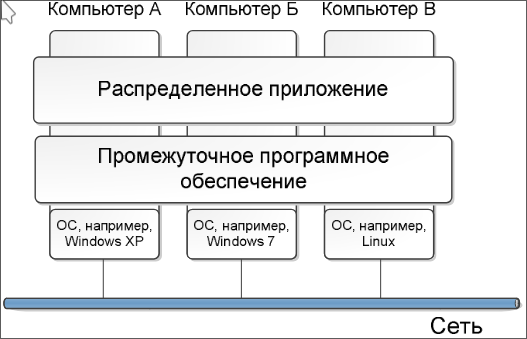
\includegraphics[scale=0.4]{inc/distr-arch.png}
  \caption{Слои программного обеспечения РВС \cite{radchenko2012}}
  \label{fig:distributed-architecture}
\end{figure}

Для того чтобы система выглядела пользователю как единая, применяют следующие
виды прозрачности \cite{radchenko2012}:

\begin{itemize}
    \item \textbf{прозрачность доступа к ресурсам} — пользователи не должны
    замечать различий в способах представления данных и методах доступа;
    \item \textbf{прозрачность размещения} — физическое расположение ресурса не
    влияет на работу пользователя;
    \item \textbf{прозрачность репликации} — наличие нескольких копий ресурса
    скрывается от клиента;
    \item \textbf{прозрачность параллельного доступа} — одновременное
    использование ресурса разными клиентами не должно требовать дополнительной
    координации
    со стороны пользователя;
    \item \textbf{прозрачность отказов} — выход из строя узла или отдельного
    ресурса не должен приводить к потере данных или прекращению работы
    приложений.
\end{itemize}

\subsection{Проблемы согласованности и отказоустойчивости}

Ключевая теоретическая трудность распределённых систем заключается в достижении
согласованного состояния между узлами при наличии сбоев и асинхронности
коммуникаций. Классический результат Фишера—Линч—Патерсона (FLP) показывает
невозможность детерминированного консенсуса в полностью асинхронной системе
даже при наличии одного отказавшего процесса \cite{flp1985}. Этот результат не
делает построение практических систем невозможным, но подчёркивает
необходимость явных инженерных допущений (таймеры, частичная синхронность,
перезапуски) и использования алгоритмов, которые обеспечивают безопасность
(safety) при любой динамике, а живучесть (liveness) — при выполнении
ограниченных условий синхронизации \cite{lynch1996,birman2012}.

Отказоустойчивость в прикладном смысле означает сохранение доступности и
корректности при отказах отдельных узлов и временной недоступности
коммуникационных каналов. Для этого применяются репликация состояния, изоляция
отказов, автоматическое восстановление и предотвращение одновременного
существования нескольких лидеров (split-brain). Наиболее распространённым
конструктом является реплицированная машина состояний: клиентоориентированные
операции записываются в общий лог и детерминированно применяются всеми
репликами в одном и том же порядке, что обеспечивает эквивалентность состояний
\cite{coulouris2012,lynch1996}.

\subsection{Роль алгоритмов консенсуса}

Алгоритм консенсуса описывает работу распределенной системы, которая при наличии
нескольких процессов, начинающих работу с некого начального состояния, переводит
все процессы в одинаковое состояние. Чтобы алгоритм консенсуса был корректным,
должны выполняться следующие условия \cite{petrov}:

\begin{itemize}
    \item Согласованность. Принимаемое протоколом решение должно быть единодушным:
        каждый процесс  выбирает некоторое значение, которое должно быть
        одинаковым для всех процессов.
    \item Действительность. Согласованное значение должно быть предложено одним
        из процессов. Т.е. это не может быть некое произвольное значение.
    \item Окончательность. Согласованность принимает окончательный характер после
        того, как уже не остается процессов, не достигших состояния принятия решения.
\end{itemize}

Алгоритмы консенсуса должны учитывать множество источников недетерминизма:
потери и задержки сообщений, дублирование пакетов, разделение сети (network
partitions), а также отказы узлов как с завершением работы (crash-stop), так и
с восстановлением (crash-recovery) \cite{birman2012, kleppmann2017}. Для
корректной работы требуется наличие \textbf{кворума} — подмножества узлов,
достаточного для принятия решения. Обычно кворумом является простое большинство
($\lceil (N/2) + 1 \rceil$ узлов из $N$), что обеспечивает устойчивость к
отказу меньшей половины кластера.

Особую роль консенсус играет в системах, где требуется \textbf{строгая
согласованность} (linearizability): каждая операция должна выглядеть так, как
будто она выполняется моментально в некоторый момент времени между своим
вызовом и ответом. Без консенсуса реализация таких гарантий невозможна, так как
неконтролируемые сетевые задержки могут привести к рассогласованию состояний.

Современные алгоритмы консенсуса (Paxos, Raft, Zab) используют
похожую модель:
\begin{itemize}
    \item выбор координатора (лидера), который упорядочивает запросы;
    \item протокол подтверждений, гарантирующий, что запись
    добавлена в кворум узлов;
    \item фиксацию (commit), после которой результат становится видим
    всем участникам и может быть применён к состоянию системы.
\end{itemize}

Таким образом, алгоритмы консенсуса служат «системной шиной» для распределённых
приложений, скрывая сложность сетевых сбоев и обеспечивая единообразие работы
кластера. Именно поэтому корректность и эффективность этих алгоритмов
критически важны для построения надёжных распределённых систем.

\subsection{Обоснование выбора алгоритма консенсуса Raft}

Выбор алгоритма консенсуса является ключевым этапом при проектировании
отказоустойчивых распределённых систем. От него напрямую зависят сложность
реализации, удобство сопровождения кода, а также прозрачность поведения системы
для разработчиков и администраторов. Исторически первой широко известной и
формально доказанной реализацией консенсуса был алгоритм Paxos, предложенный
Лампором. Paxos обладает строгими теоретическими гарантиями безопасности и
живучести, но отличается сложной и трудно воспринимаемой спецификацией, что не
раз отмечалось в инженерной литературе и практике промышленной разработки
\cite{lamport2001paxos}. Разработка корректной и полной реализации
Paxos требует значительных усилий и глубокого понимания формальных инвариантов,
что повышает риск ошибок при практическом применении.

Алгоритм Raft был создан как ответ на эту проблему. Его основной целью было
повышение «понимаемости» протокола консенсуса без ущерба для гарантий
корректности. Авторы Raft отмечают, что понимаемость протокола напрямую влияет
на вероятность корректной реализации и снижает риск скрытых ошибок, которые
могут проявиться лишь при сбоях или высокой нагрузке \cite{ongario2014}. Raft
декомпозирует задачу консенсуса на несколько изолированных подпроблем (выбор
лидера, репликация логов, гарантия безопасности логов), что облегчает
рассуждения об инвариантах системы и значительно упрощает обучение
разработчиков.

Дополнительным аргументом в пользу Raft является его популярность и зрелость
реализации в открытых проектах. Сегодня Raft используется во многих
промышленных системах — например, в etcd (сервис конфигурации в Kubernetes),
Consul, TiKV, RethinkDB, Tarantool, что подтверждает его практическую
применимость и широкую проверку в реальных условиях эксплуатации. Благодаря
этому для Raft существует обширная документация, научные статьи, что сокращает
затраты времени на разработку и уменьшает вероятность внедрения ошибок на
ранних этапах.

С точки зрения проектируемой системы, Raft является оптимальным выбором,
так как:
\begin{itemize}
    \item обеспечивает строгую согласованность данных и устойчивость
    к отказу меньшинства узлов;
    \item обладает ясной архитектурой и хорошо описанными сценариями
    поведения при сбоях;
    \item имеет многочисленные реализации и практические рекомендации
    по настройке, что упрощает написание собственной реализации;
    \item подходит для систем с выделенным лидером, где клиентские
    запросы упорядочиваются в единую последовательность,
    что соответствует выбранной архитектуре (узлы Raft управляют
    логом операций и синхронизируют его между собой).
\end{itemize}

Таким образом, Raft предоставляет необходимый баланс между теоретической
строгостью и инженерной простотой, снижая риск некорректной реализации и
ускоряя процесс разработки. Это делает его наиболее подходящим протоколом
консенсуса для решения поставленных в работе задач по обеспечению
отказоустойчивости и согласованности распределённых вычислений.

    \section{Raft}

В Raft каждый узел хранит локально журнал команд, исполняемых конечным автоматом.
Так как все процессы получают одинаковые входные данные и применяют идентичные
команды в одном и том же порядке, их конечные автоматы приходят к одинаковому
состоянию. Одно из отличий Raft заключается в том, что роль лидера здесь
вынесена на первый план: он координирует репликацию и манипуляции над конечным
автоматом. С этой точки зрения Raft схож с Мульти-Паксосом и атомарной рассылкой:
среди узлов выбирается лидер, который принимает решения и задаёт упорядочение
сообщений.

Алгоритм Raft определяет три основные роли:

\begin{itemize}
    \item Кандидат (candidate): Узел, который пытается стать лидером. Он набирает
        голоса большинства узлов. Если выборы не приводят к явному победителю,
        запускается новый период и процесс голосования повторяется.
    \item Лидер (leader): Временный управляющий кластером, обрабатывающий запросы
        клиентов и взаимодействующий с реплицируемым конечным автоматом. Лидер
        выбирается на определённый период, который идентифицируется возрастающим
        номером. Если лидер перестаёт отвечать или подозревается в отказе,
        начинается процедура переизбрания.
    \item Последователь (follower): Пассивный участник, хранящий записи журнала
        и реагирующий на запросы от лидера и кандидатов. По сути, в Raft он
        объединяет в себе функции акцептора и ученика из Паксоса. Каждый узел
        стартует в роли последователя.
\end{itemize}

Чтобы добиться упорядочения без жёсткой синхронизации часов, в Raft используются
периоды (эпохи, термы), в течение которых существует только один лидер. Каждый
период имеет уникальный номер, а команды внутри периода получают дополнительный
индекс. Узлы могут по-разному воспринимать текущий период (например, если они
пропустили этап выборов), но каждая отправляемая команда указывает номер
периода \cite{ongario2014}. Если узел видит период с более высоким номером, он
обновляет своё значение периода.

Процесс выбора лидера инициируется, когда последователь не получает подтверждений
от текущего лидера, полагая, что тот вышел из строя. В этом случае последователь
переходит в состояние кандидата и собирает голоса большинства узлов, стремясь
стать новым лидером.

На рис. \ref{fig:raft} приведена схема раунда Raft.

\begin{figure}
  \centering
  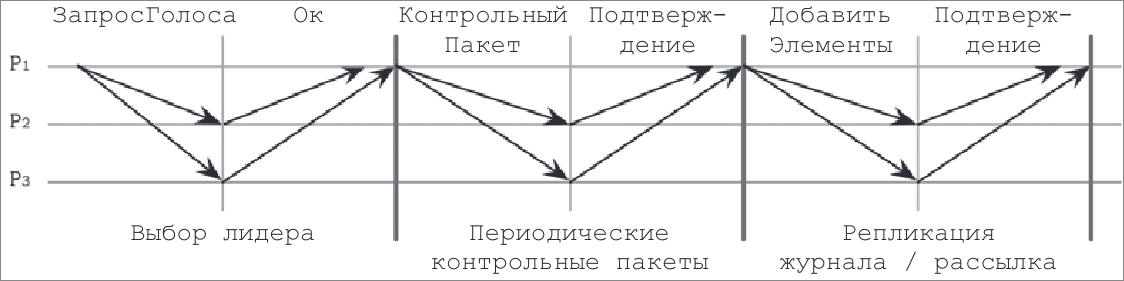
\includegraphics[scale=0.4]{inc/raft.png}
  \caption{Схема раунда Raft}
  \label{fig:raft}
\end{figure}

\begin{itemize}
    \item Выбор лидера. Когда узел-кандидат (P1 на рисунке) решает стать лидером,
        он рассылает остальным участникам сообщение $ЗапросГолоса$, содержащее свой
        период, последнюю известную ему информацию о периоде, а также идентификатор
        самой свежей записи в журнале, которую он видел. Если кандидат получает
        большинство голосов, он становится лидером на текущий период. При этом
        каждый узел может отдать голос лишь одному кандидату.
    \item Периодические контрольные пакеты. Для поддержания жизнеспособности
        системы лидер с определённой периодичностью отправляет контрольные
        пакеты всем последователям, тем самым подтверждая своё лидерство. Если
        последователь не получает такие пакеты в течение «тайм-аута выборов»,
        он предполагает сбой лидера и инициирует новый процесс голосования.
    \item Репликация. Лидер может неоднократно пополнять реплицируемый журнал,
        отправляя сообщение $ДобавитьЭлементы$, где указывает период лидера,
        индекс и период последней зафиксированной записи, а также одну или
        несколько новых записей для сохранения.
\end{itemize}

\subsection{Роль лидера в Raft}

Лидер может быть выбран только среди узлов, содержащих все актуальные записи.
Если в процессе выборов журнал последователя более актуальный, чем у кандидата,
то голос за этого кандидата не отдается.

Для победы в голосовании кандидат должен получить большинство голосов. Поскольку
записи реплицируются строго по порядку, достаточно сравнить идентификаторы последних
записей. После избрания лидер начинает принимать запросы от клиентов и реплицирует
их на своих последователей. Для этого он добавляет запись в свой журнал и
одновременно отправляет её всем последователям.

Когда последователь получает сообщение о добавлении записей, он вносит эти
записи в локальный журнал и отправляет подтверждение, сообщая лидеру, что данные
сохранены. Как только лидер получает достаточное количество подтверждений, запись
считается зафиксированной и помечается соответствующим образом в его журнале.

Поскольку лидером может стать только узел с наиболее актуальными данными,
последователь не отправляет ему обновления. Записи журнала передаются
только в одном направлении — от лидера к последователям.

На рисунке \ref{fig:raft-consensus} представлен пример раунда достижения
консенсуса, в котором узел P1 выступает в роли лидера с наиболее актуальной
информацией. Лидер выполняет алгоритм, реплицируя записи на своих последователей
и фиксируя их после получения подтверждений. Фиксация одной записи автоматически
фиксирует все предшествующие записи в журнале. Решение о фиксации может принимать
только лидер. Каждая запись в журнале имеет идентификатор периода (терма, указан в
верхнем правом углу записи) и индекс, определяющий её позицию в журнале.
Зафиксированные записи гарантированно реплицируются на кворум узлов, что
позволяет безопасно применять их к конечному автомату в порядке их добавления.

\begin{figure}
  \centering
  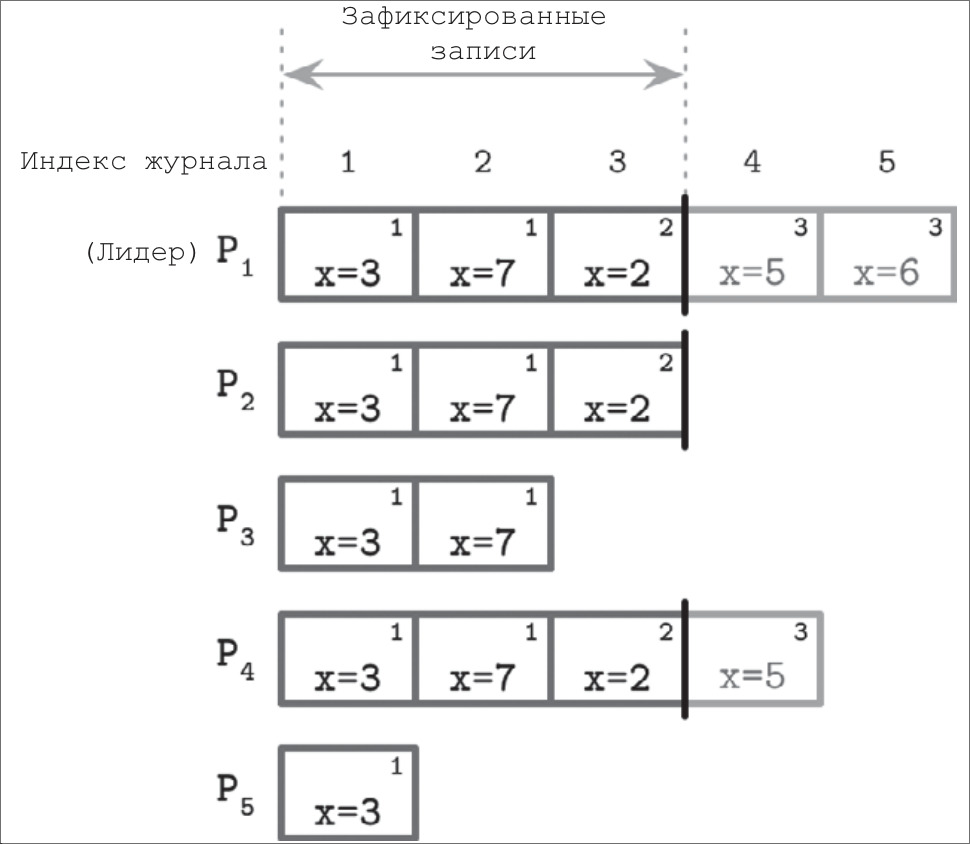
\includegraphics[scale=0.4]{inc/raft-consensus.png}
  \caption{Конечный автомат алгоритма Raft}
  \label{fig:raft-consensus}
\end{figure}

\subsection{Сценарии отказов}

Когда несколько последователей решают стать кандидатами, но ни один из них не
может набрать большинство голосов, такая ситуация называется "разделенным
голосованием". Чтобы снизить вероятность таких случаев, алгоритм Raft применяет
рандомизированные таймеры. Это позволяет одному из кандидатов начать следующий
этап выборов раньше других, получить достаточное количество голосов и быть
избранным, пока остальные кандидаты находятся в ожидании. Такой подход ускоряет
процесс выборов, исключая необходимость дополнительной координации между кандидатами.

Если последователи отключаются или задерживают ответы, лидер обязан
предпринимать дополнительные попытки доставки сообщений. Если подтверждение от
узлов не поступает в ожидаемый срок, лидер повторно отправляет сообщения.

Благодаря уникальным идентификаторам, присваиваемым реплицируемым записям,
порядок в журнале остается неизменным, даже при повторной доставке сообщений.
Последователи устраняют дублирующие записи, основываясь на их порядковых номерах,
что предотвращает нежелательные эффекты от повторных отправок. Также порядковые
номера используются для соблюдения хронологии в журнале: последователь отклоняет
записи с более высокими номерами, если предыдущие записи не совпадают с
его журналом. Если две записи из разных журналов имеют одинаковые идентификаторы
и индексы, то они хранят одну и ту же команду, а все предшествующие им записи
идентичны.

Для обнаружения сбоев лидер отправляет последовательным узлам контрольные
сообщения, подтверждая тем самым активность своего периода. Если один из узлов
замечает, что текущий лидер перестал отвечать, он инициирует процедуру выборов.
Новый лидер восстанавливает состояние кластера, определяя последнюю согласованную
запись (то есть запись с наибольшим номером, которую разделяют лидер и последователь).
Он приказывает узлам удалить все незафиксированные записи после этой точки и
реплицирует актуальные записи из своего журнала. Лидер не удаляет и не
перезаписывает собственные записи, а только добавляет новые.

Таким образом, Raft предоставляет следующие гарантии:

\begin{itemize}
    \item Только один лидер может быть избран одновременно на заданный период (терм);
        в течение одного периода не может быть двух активных лидеров;
    \item Лидер не удаляет и не переупорядочивает содержимое журнала; он только
        добавляет новые сообщения к нему;
    \item Зафиксированные записи в журнале гарантированно присутствуют в журналах
        для последующих лидеров;
    \item Все сообщения однозначно идентифицируются по идентификаторам сообщений
        и периодов; ни текущий, ни последующие лидеры не могут повторно использовать
        один и тот же идентификатор для другой записи.
\end{itemize}


    \section{Проектирование архитектуры системы}

\subsection{Общая архитектура системы}

\subsubsection{Роли узлов}

На верхнем уровне архитектуры выделяются два класса узлов: \emph{узлы
консенсуса (Raft-узлы)} и \emph{вычислительные узлы (workers)}. Такое
разделение соответствует распространённой практике отделения \emph{control
plane} (координация, согласование состояния, диспетчеризация) от
\emph{data/compute plane} (непосредственное выполнение пользовательских задач)
\cite{coulouris2012}.

Raft-узлы формируют кластер, поддерживающий реплицированную машину состояний,
принимают клиентские запросы, выполняют проверку/валидацию, принимают решения о
постановке задач в очередь и о распределении задач по воркерам, а также
обеспечивают линейризуемую (или близкую к ней) семантику наблюдения состояния.

Воркеры, в свою очередь, реализуют только «полезную работу»: исполняют выданные
задания в соответствии с политикой планировщика, периодически отчитываются о
прогрессе и возвращают результаты.

Архитектура приложения приведена на рис.~\ref{fig:arch-overview}.

\begin{figure}
  \centering
  \includegraphics[scale=0.4]{inc/arch-overview.png}
  \caption{Высокоуровневая архитектура приложения}
  \label{fig:arch-overview}
\end{figure}

Данный подход минимизирует связанность компонентов: все операции записи в
«истину состояния» проходят через кластер Raft, а вычислительный контур
остаётся тонким и легко масштабируемым.

Это упрощает развитие системы (изменения протокола, эволюцию форматов,
миграции), повышает управляемость и упрощает доказательство корректности, так
как инварианты безопасности сосредоточены в одном месте — в реплицированной
машине состояний.

\subsubsection{Потоки управления и данные}

Клиент взаимодействует только с кластером Raft (запросы могут быть приняты
любым узлом и переадресованы лидеру). Каждая операция, которая влияет на
состояние системы (создание/отмена задания, изменение приоритета, отметка
результата), сначала записывается в лог кластера, подтверждается кворумом узлов
и \emph{только затем} применяется к машине состояний.

Из машины состояний изменения транслируются в модуль диспетчеризации (Task
manager), который назначает задания конкретным воркерам.

Обратный поток (результаты) также фиксируется через Raft перед тем, как станет
видимым для клиента.

Такая схема обеспечивает:
\begin{itemize}
    \item детерминированный порядок событий;
    \item устойчивость к повторам и сетевым артефактам за счёт идемпотентных
    идентификаторов задач;
    \item возможность повторного назначения задач при сбоях воркеров без
    нарушения согласованности.
\end{itemize}

\subsubsection{Обоснование отсутствия прямых связей между клиентом и рабочим узлом}

Исключение прямого клиентского трафика на воркеры и запрет горизонтальных
коммуникаций между воркерами снижает сложность системы и радиус отказа:

\begin{itemize}
  \item \textbf{Границы доверия и безопасность.} Все проверки
  аутентификации/авторизации, квоты, контроль нагрузки и согласование политик
  происходят в одном месте (в кластере Raft), что уменьшает поверхность атаки и
  упрощает аудит.
  \item \textbf{Единая точка сериализации.} Централизация записи в лог
  предотвращает расхождение состояний при разделениях сети и сбоях; воркеры не
  принимают решений, влияющих на глобальную консистентность.
  \item \textbf{Простота воркеров.} Воркеры могут оставаться без состояния
  (stateless) или слабосвязными по состоянию; замена/масштабирование происходит
  без координации между ними, что упрощает эксплуатацию.
  \item \textbf{Управляемое масштабирование.} Планирование, балансировка
  сосредоточены в кластере Raft; добавление воркеров линейно увеличивает
  пропускную способность без изменения протоколов согласования.
\end{itemize}

\subsubsection{Отказоустойчивость и модель сбоев}

Система проектируется под модель сбоев crash-stop/crash-recovery и частичной
синхронности сети.

Кластер Raft обеспечивает безопасность (отсутствие противоречивых коммитов) при
любой динамике и живучесть при выполнении допущений о времени
\cite{ongario2014}. Отказ отдельного воркера не влияет на целостность:
незавершённые задания остаются зафиксированными в состоянии и могут быть
переназначены. При отказе лидера выполняется переизбрание; после выбора нового
лидера система продолжает обслуживание запросов, как только будет достигнут
кворум. Такая конфигурация позволяет сохранять работоспособность при
недоступности до $\lfloor (N-1)/2 \rfloor$ узлов кластера консенсуса (для $N$ —
числа Raft-узлов), что является стандартной кворумной гарантией
\cite{lynch1996}.


\subsubsection{Масштабирование и управление нагрузкой}

Архитектура поддерживает независимое масштабирование плоскостей:
\begin{itemize}
  \item \textbf{Горизонтальный рост вычислительных мощностей.} Добавление воркеров
  увеличивает суммарные вычислительные мощности без влияния на алгоритм
  консенсуса.
  \item \textbf{Стабильность.} Количество Raft-узлов остаётся небольшим (обычно
  3–5) для минимизации латентности кворума и времени выборов
  \cite{ongario2014}.
\end{itemize}

\subsubsection{Рассмотренные альтернативы}

Были рассмотрены альтернативные топологии:

\begin{itemize}
\item прямое взаимодействие клиента с воркерами;
\item полно-связанная p2p-сетка воркеров с децентрализованным согласованием;
\item объединение ролей (каждый воркер — участник консенсуса).
\end{itemize}

От первого варианта отказались из-за роста поверхности ошибок и сложности
обеспечения глобальной согласованности. Второй вариант усложняет доказательство
корректности и эксплуатацию (динамика членства, маршрутизация, «горячие»
ключи). Третий ухудшает масштабирование: увеличение количества участников
консенсуса повышает латентность кворума и время выбора лидера.

Предложенная архитектура сохраняет консенсус компактным и управляемым, а
вычисления — эластичными и дешёвыми в масштабировании.

\subsection{Архитектура Raft узлов}

Каждый узел кластера Raft содержит несколько функциональных модулей,
взаимодействие которых обеспечивает корректную обработку запросов и поддержание
согласованного состояния всей системы. Архитектура узла изображена на
рис.~\ref{fig:arch-overview}.

\begin{figure}
  \centering
  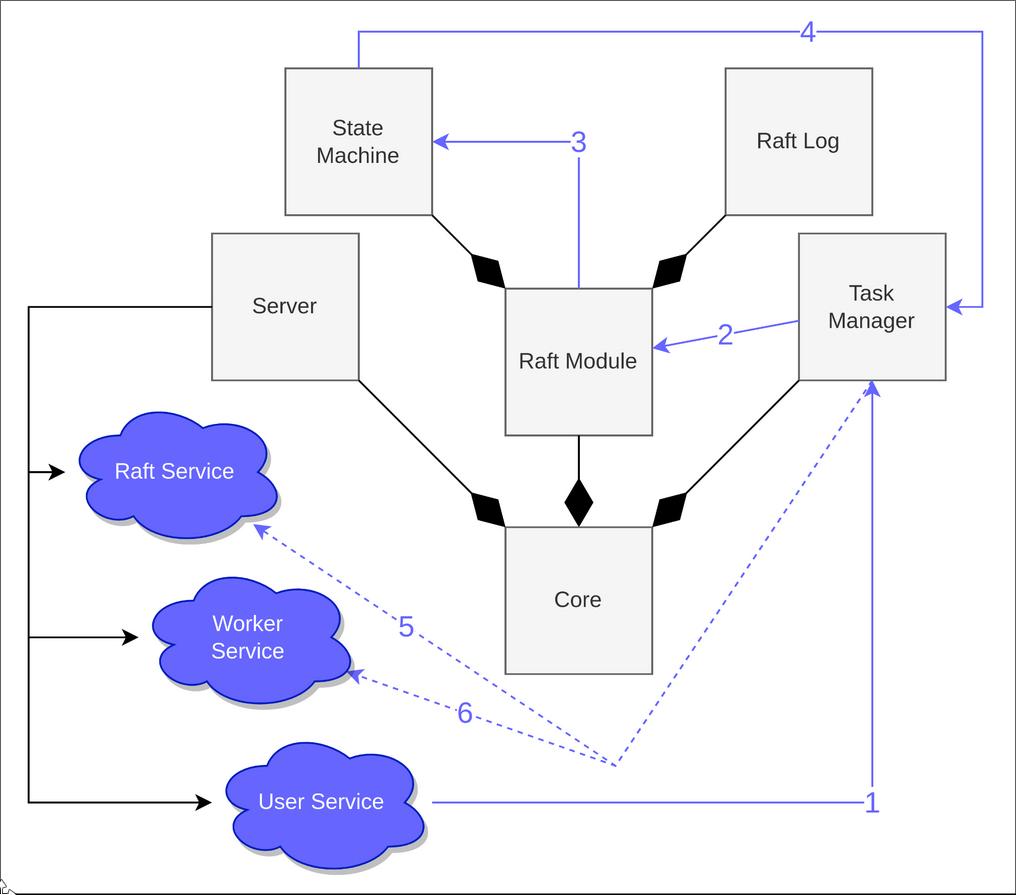
\includegraphics[scale=0.35]{inc/raft-arch.png}
  \caption{Архитектура Raft узла}
  \label{fig:arch-overview}
\end{figure}

Поток обработки клиентского запроса начинается с поступления данных на
\textbf{серверный модуль} узла-лидера. Сервер принимает запросы от клиентов и
маршрутизирует их во внутренние сервисы. В частности, запросы, связанные с
постановкой новых заданий на выполнение, направляются в
\textbf{пользовательский сервис (User Service)}, зарегистрированный в сервере.
Этот сервис выполняет первичную валидацию и подготовку данных, после чего
передаёт их в \textbf{менеджер заданий (Task Manager)}. Задача менеджера —
выбрать подходящий рабочий узел (worker) для выполнения поступившей задачи,
исходя из состояния системы, доступности ресурсов и стратегий планирования.

Поскольку система должна сохранять корректность работы даже при сбоях
отдельных узлов, Task Manager не отправляет задание воркеру напрямую.
Вместо этого сформированная операция передаётся в
\textbf{модуль Raft}, который отвечает за репликацию и согласование
состояния между всеми узлами кластера. Raft-модуль добавляет операцию
в \textbf{журнал Raft (Raft Log)}, который хранит все ещё не
зафиксированные изменения состояния. В рамках механизма Raft эти записи
реплицируются на все узлы кластера при очередных heartbeat-сообщениях
лидера.

Когда большинство (кворум) узлов подтверждает успешную запись данных в свои
локальные логи, лидер выполняет \textbf{коммит (commit)} — операцию переноса
записи в \textbf{машину состояний (State Machine)}. Машина состояний
представляет собой детерминированный автомат, который преобразует
последовательность закоммиченных операций в текущее состояние системы. За счёт
применения одной и той же последовательности команд на каждом узле достигается
консенсус — все реплики приходят к одинаковому результату независимо от того,
какой узел является лидером.

После того как операция фиксируется в машине состояний лидера, Task Manager
получает сигнал о возможности безопасного выполнения задания. На этом этапе
задание отправляется выбранному воркеру. Результат выполнения также проходит
через Raft: при завершении работы воркер формирует ответ, который реплицируется
и коммитится аналогично исходному запросу. Лишь после этого результат считается
подтверждённым и возвращается клиенту, что гарантирует согласованность даже при
отказах в момент ответа.

Ключевым элементом узла является \textbf{ядро (Core)}, которое выполняет роль
интеграционного слоя между модулями. Core отвечает за инициализацию и
завершение работы компонентов, координирует обмен сообщениями между ними и
предоставляет единый интерфейс для внешнего управления узлом.

Такая архитектура обеспечивает согласованное и детерминированное поведение
системы при сбоях, гарантирует, что любая операция либо применена на
большинстве узлов, либо будет проигнорирована. Система остаётся работоспособной
до тех пор, пока доступно более половины узлов кластера, что является базовым
требованием алгоритмов кворумного консенсуса.

\subsection{Архитектура клиентской части}

Клиентская часть системы обеспечивает пользователю удобный интерфейс
для постановки задач на выполнение и получения результатов.
Основными компонентами клиентской стороны являются:
\begin{itemize}
    \item \textbf{Конфигурационные данные задачи} — входные параметры,
    описывающие вычислительную задачу, хранятся в формате JSON
    (например, \texttt{data.json}). Такой формат выбран благодаря
    читаемости, простоте валидации и широкому распространению
    в экосистемах различных языков.
    \item \textbf{Библиотека задачи} — бинарный модуль
    (\texttt{libtask.so}), содержащий реализацию функции обработки данных.
    Такой подход позволяет передавать не только статические входные данные,
    но и сам алгоритм, который должен быть исполнен на воркере.
    \item \textbf{Клиентское приложение (CLI)} — консольная утилита,
    служащая интерфейсом между пользователем и распределённой системой.
    CLI принимает указанные входные файлы, сериализует их в формат,
    подходящий для сетевой передачи, и формирует запрос к кластеру Raft.
\end{itemize}

Процесс взаимодействия клиента с системой проходит следующие этапы (см.
рис.~\ref{fig:client-arch}):
\begin{enumerate}
    \item Пользователь передаёт клиенту \texttt{data.json} и
    динамическую библиотеку \texttt{libtask.so}, после чего CLI
    формирует запрос, содержащий данные задачи и код её исполнения,
    и отправляет его в кластер Raft.
    \item Лидер кластера принимает запрос, реплицирует его
    и передаёт в подсистему диспетчеризации, которая назначает
    задачу конкретному рабочему узлу. В запросе указывается
    уникальный идентификатор задачи для обеспечения идемпотентности.
    \item Клиент воркера получает задание и передаёт его на выполнение
    в среду исполнения, где подгружается \texttt{libtask.so} и
    запускается соответствующая функция с параметрами из \texttt{data.json}.
    После завершения выполнения результат формируется в сериализованном
    виде и отправляется обратно в кластер Raft для фиксации в состоянии.
    \item После коммита результата в реплицированной машине состояний
    лидер Raft уведомляет клиента о завершении работы. CLI принимает
    ответ, сохраняет результат локально либо выводит пользователю
    в удобной форме.
\end{enumerate}

\begin{figure}
  \centering
  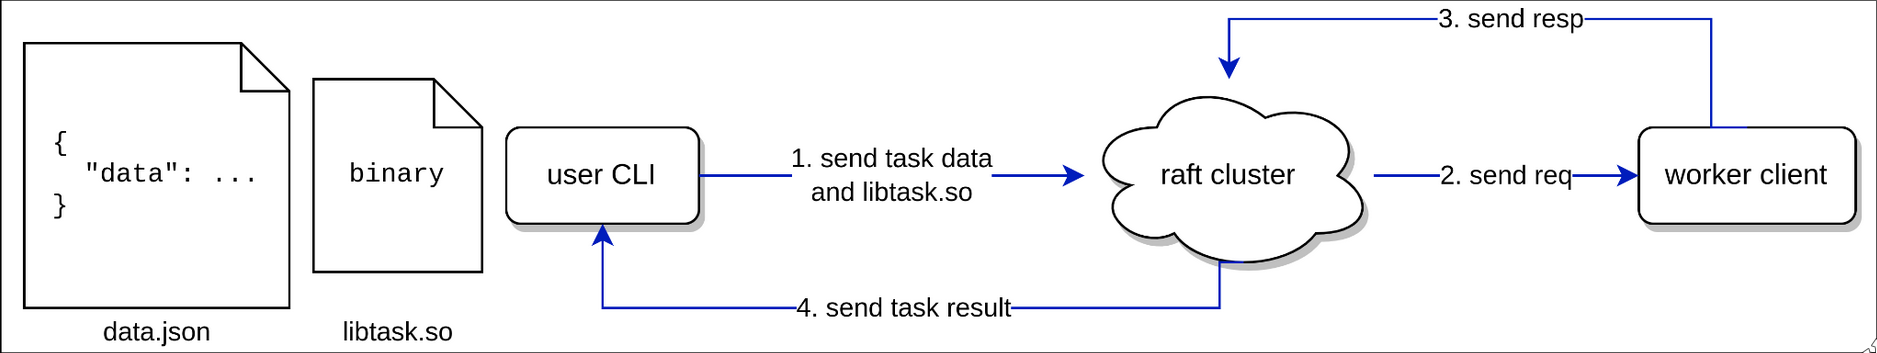
\includegraphics[scale=0.25]{inc/client-arch.png}
  \caption{Взаимодействие клиента с кластером}
  \label{fig:client-arch}
\end{figure}

Данная архитектура клиентской части обладает рядом преимуществ:
\begin{itemize}
    \item \textbf{Универсальность.} Клиент не привязан к конкретному
    типу задач — любое вычисление, представленное в виде бинарной
    библиотеки с единым интерфейсом, может быть передано в систему.
    \item \textbf{Минимальные зависимости.} Клиент реализован как
    лёгкая утилита, не требующая сложной конфигурации;
    это упрощает её развёртывание и интеграцию в CI/CD.
    \item \textbf{Надёжность.} Все этапы (от постановки задачи до
    получения ответа) проходят через механизм Raft, что гарантирует
    сохранность данных даже при сбоях сети или падении узлов.
\end{itemize}

Таким образом, клиентская часть системы выступает удобным
и унифицированным интерфейсом, который инкапсулирует сложность
взаимодействия с распределённой инфраструктурой и позволяет
пользователю сосредоточиться на определении вычислительных задач
и анализе результатов.

\subsection{Архитектура вычислительного узла}

Вычислительный узел предназначен для непосредственного выполнения задач,
поступающих из кластера Raft, и возврата результатов их обработки. Архитектура
воркера организована таким образом, чтобы обеспечить изоляцию вычислений,
устойчивость к сбоям и минимальное влияние выполняемой задачи на стабильность
основной службы.

Ключевые компоненты вычислительного узла:
\begin{itemize}
    \item \textbf{Главный процесс (main)} — точка входа, отвечающая за
    инициализацию среды, запуск клиента воркера и менеджера процессов. Главный
    процесс контролирует жизненный цикл остальных компонентов и обеспечивает их
    перезапуск при сбоях.
    \item \textbf{Клиент воркера (worker client)} — процесс, который
    поддерживает постоянное соединение с кластером Raft, принимает задания на
    выполнение и уведомляет менеджер о необходимости запуска вычислительных
    контейнеров.
    \item \textbf{Менеджер (manager)} — отдельный процесс, отвечающий за
    создание изолированных рабочих процессов (\textbf{mayfly}), которым
    передаётся выполнение конкретных задач. Такой подход снижает риск
    повреждения памяти или зависания основного сервиса из-за некорректного кода
    задачи.
    \item \textbf{Mayfly-процесс} — лёгкий дочерний процесс, который выполняет
    задачу. На этапе инициализации загружает указанную динамическую библиотеку,
    выполняет функцию обработки данных и формирует результат.
\end{itemize}

Поток выполнения задачи организован следующим образом (см.
рис~\ref{fig:worker-arch}):

\begin{enumerate}
    \item \textbf{Приём запроса.} Worker client получает задание
    из кластера Raft и подтверждает его приём.
    \item \textbf{Создание рабочего процесса.} Worker client
    отправляет запрос менеджеру на создание нового mayfly-процесса.
    Менеджер выполняет \texttt{fork()}, создавая изолированный процесс.
    \item \textbf{Загрузка библиотеки.} Mayfly-процесс подгружает
    указанную пользователем библиотеку задачи (по имени, переданному
    в запросе).
    \item \textbf{Выполнение задачи.} Обработка входных данных
    производится внутри mayfly-процесса.
    В случае ошибки или аварийного завершения процесс завершается
    без влияния на основной клиент воркера.
    \item \textbf{Отправка результата.} После завершения выполнения
    результат возвращается менеджеру, который передаёт его обратно
    в worker client.
    \item \textbf{Репликация результата.} Worker client формирует
    ответ и отправляет его в кластер Raft для фиксации в
    реплицированной машине состояний.
\end{enumerate}

\begin{figure}
  \centering
  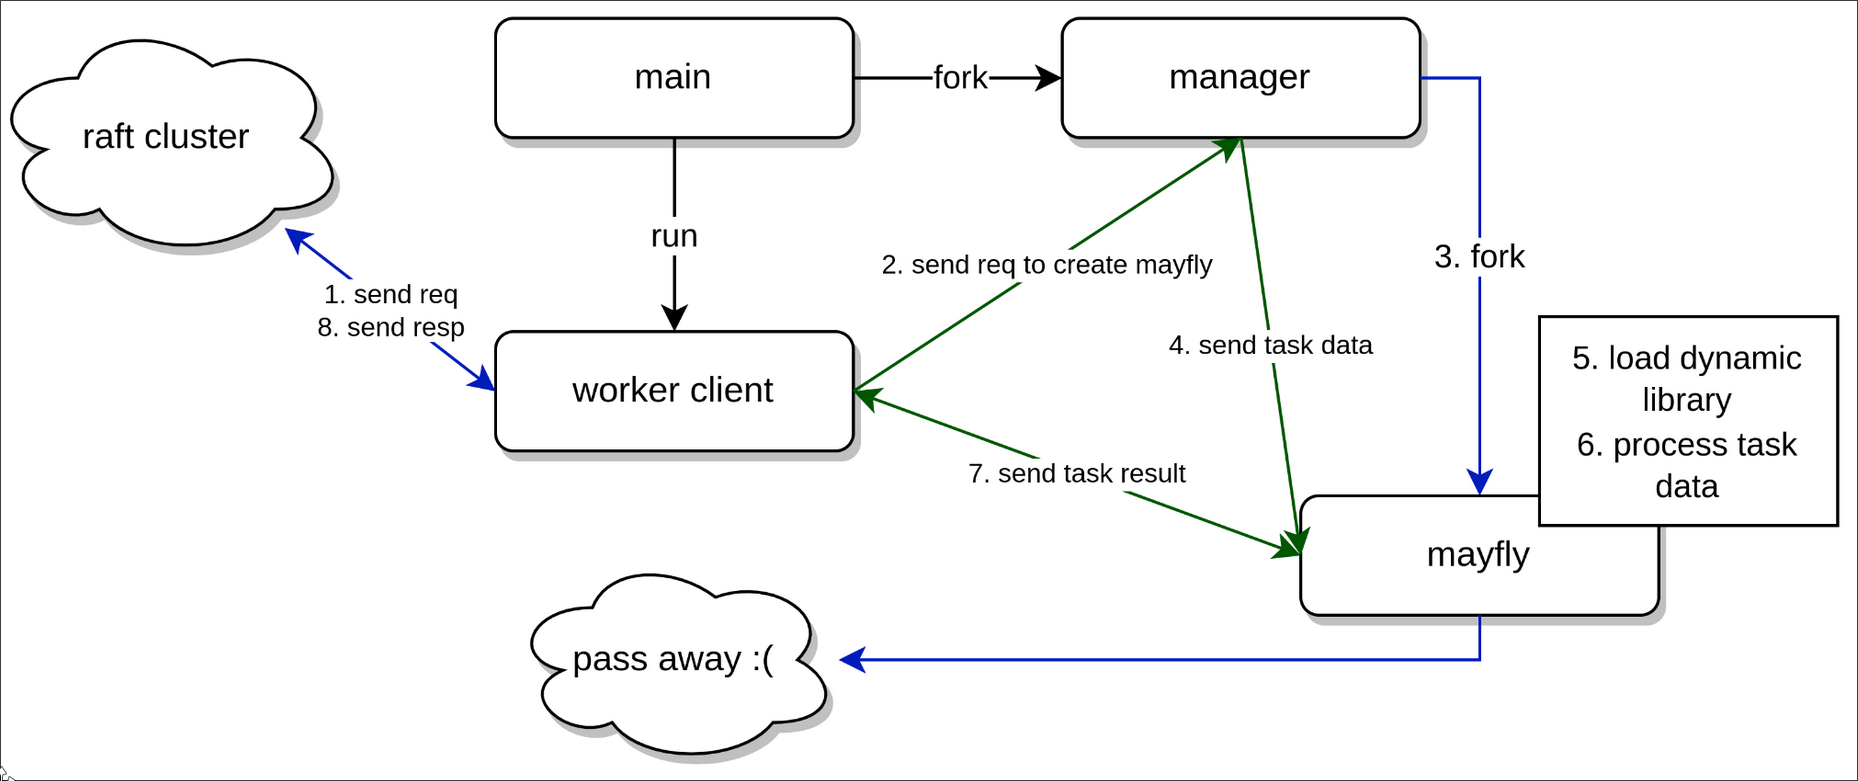
\includegraphics[scale=0.25]{inc/worker-arch.png}
  \caption{Взаимодействие вычислительного узла с кластером}
  \label{fig:worker-arch}
\end{figure}

Архитектура поддерживает модель «одно задание — один процесс», что
обеспечивает:

\begin{itemize}
    \item \textbf{Изоляцию исполнения}: сбой в задаче не влияет
    на остальные процессы воркера;
    \item \textbf{Высокую отказоустойчивость}: при завершении
    дочернего процесса менеджер может корректно обработать сбой,
    зарегистрировать ошибку и при необходимости запросить
    повторное выполнение через кластер;
    \item \textbf{Простоту очистки ресурсов}: после завершения работы
    mayfly-процесс уничтожается вместе с выделенными ресурсами,
    исключая утечки памяти.
\end{itemize}

Такое построение вычислительного узла обеспечивает гибкость и устойчивость всей
системы, позволяя безопасно выполнять пользовательский код, динамически
масштабировать количество обрабатываемых задач и гарантировать возврат
результата даже при частичных сбоях.

    \section{Реализация системы распределенных вычислений}

В данном разделе описан выбор технологического стека и его роль в реализации
распределённой системы. Подробно обоснован выбор gRPC и Protocol Buffers как
основы сетевого взаимодействия, обеспечивающих строгую типизацию,
производительность и удобство сопровождения кода. Далее рассмотрена реализация
Raft-узла как центрального компонента кластера, включая структуру лога, машину
состояний с механизмом снепшотов, серверный модуль и менеджер заданий.
Приведены ключевые аспекты работы клиентского приложения, включая формат
конфигурационных файлов и двунаправленный потоковый протокол взаимодействия, а
также описана организация вычислительных узлов, их взаимодействие с кластером и
обработка сбоев. В совокупности раздел демонстрирует, каким образом выбранные
технологии и архитектурные решения обеспечивают согласованность состояния,
отказоустойчивость и удобство масштабирования всей системы.

В приложении А приведен протокол всех частей распределенной вычислительной
системы, в приложении Б находится полная UML-диаграмма классов всех частей. В
проекте Abeille \cite{abeille} можно найти полный исходный код.

\subsection{Выбор технологий и инструментов}

Для реализации сетевого взаимодействия в системе был выбран современный
стек \textbf{gRPC + Protocol Buffers}, который обеспечивает эффективную
и строго типизированную коммуникацию между узлами.
gRPC представляет собой высокопроизводительный фреймворк для удалённых
вызовов процедур (Remote Procedure Call, RPC), разработанный компанией Google.
Он использует протокол HTTP/2 на прикладном уровне и TCP на транспортном,
что позволяет реализовать двунаправленные потоки, мультиплексирование
и сжатие заголовков, а также снижает накладные расходы на установку соединений.

Для описания интерфейсов gRPC использует \textbf{.proto}-файлы,
обрабатываемые компилятором Protocol Buffers, который автоматически
генерирует код клиентских и серверных заглушек на выбранных языках.
В рамках данной системы .proto-файлы служат единым источником правды
для определения всех контрактов: как между клиентом и кластером Raft,
так и между внутренними компонентами (сервер, менеджер заданий, воркеры).
Это снижает вероятность ошибок согласования интерфейсов,
упрощает сопровождение системы и повышает читаемость кода.

Использование данного стека технологий обеспечивает следующие преимущества:
\begin{itemize}
    \item \textbf{Единая модель данных:} структуры описываются
    один раз в .proto-файлах и автоматически транслируются
    в типобезопасные объекты для всех участвующих компонентов.
    \item \textbf{Удобная сериализация:} поддержка как бинарного,
    так и текстового формата, что упрощает отладку и анализ
    сетевого трафика.
    \item \textbf{Эволюция протокола:} поддержка обратной и
    прямой совместимости при расширении .proto-схем, что позволяет
    постепенно обновлять компоненты системы без остановки кластера.
    \item \textbf{Высокая производительность:} низкие накладные расходы
    на передачу сообщений и эффективная поддержка параллельных
    соединений благодаря HTTP/2.
\end{itemize}

\subsection{Реализация Raft-узла}

Raft-узел является центральным элементом системы: он реализует алгоритм
консенсуса, поддерживает реплицированную машину состояний и предоставляет
интерфейсы для взаимодействия с пользователями и вычислительными узлами.
Реализация узла включает несколько взаимосвязанных компонентов: Raft-лог,
машину состояний с поддержкой снепшотов, серверный модуль, менеджер заданий и
подсистему конфигурации.

\subsubsection{Raft-лог}

Лог Raft представляет собой основной журнал команд, которые подлежат
репликации между всеми узлами кластера. После достижения кворума
запись из лога коммитится и применяется к машине состояний.
В данной реализации поддерживаются две команды:

\begin{itemize}
    \item \texttt{RAFT\_COMMAND\_ADD} — добавление новой задачи в очередь назначенных;
    \item \texttt{RAFT\_COMMAND\_MOVE} — перевод задачи в состояние завершённых.
\end{itemize}

Структура записи лога описана с использованием Protocol Buffers
(см. рис.~\ref{fig:raftlog}). Каждая запись включает тип команды,
номер терма, полезную нагрузку (упакованную в \texttt{TaskWrapper}),
а также дополнительные поля, зависящие от команды
(\texttt{AddRequest} или \texttt{MoveRequest}).
Использование Proto-схемы обеспечивает строгую типизацию,
возможность обратной совместимости при изменении формата и
автоматическую генерацию сериализаторов/десериализаторов.

\begin{figure}[h!]
    \centering
    \includegraphics[width=0.6\linewidth]{inc/raft_log_entry.png}
    \caption{Структура записи Raft-лога, определённая в формате Protocol Buffers.}
    \label{fig:raftlog}
\end{figure}

С точки зрения реализации лог представляет собой потокобезопасную обёртку над
\texttt{std::deque}. Такой выбор объясняется необходимостью обеспечения:

\begin{itemize}
    \item \textbf{Быстрого случайного доступа} по индексу (для алгоритма согласования);
    \item \textbf{Эффективного удаления элементов} как из начала
    (очистка закоммиченных записей после создания снепшота),
    так и из конца (откат неконсистентных записей при пересинхронизации).
\end{itemize}

Индексация в логе начинается с $1$; нулевой индекс считается невалидным и
используется для упрощения проверок корректности ссылок на записи.

\subsubsection{Машина состояний и механизм снепшотов}

Машина состояний реализует детерминированный автомат, который постепенно
применяет закоммиченные записи лога и формирует текущее состояние кластера. Она
хранит:

\begin{itemize}
    \item список назначенных задач;
    \item список завершённых задач;
    \item текущий номер терма и индекс последней применённой команды.
\end{itemize}

Для предотвращения бесконтрольного роста размера лога реализован механизм
\textbf{снепшотов (snapshotting)}. При достижении порога, заданного
пользователем в конфигурационном файле, машина состояний инициирует создание
снепшота: сериализует своё текущее состояние и сохраняет его на диск. Данный
процесс выполняется асинхронно, что позволяет продолжать применение новых
команд без блокировки. После успешной записи снепшота лог очищается от записей,
которые были зафиксированы в сохранённом состоянии, что ограничивает его размер
сверху.

В случае, если лидер не находит в своём логе необходимой записи для
синхронизации с отстающим узлом, он инициирует передачу ему актуального
снепшота, после чего узел может восстановить своё состояние и продолжить
репликацию с последнего зафиксированного индекса.

\subsection{Серверный модуль}

Серверный модуль инкапсулирует gRPC-сервер, принимающий запросы от:
\begin{itemize}
    \item других узлов (сервис \textbf{RaftService}: \texttt{RequestVote()},
    \texttt{AppendEntries()}, \texttt{InstallSnapshot()});
    \item клиентов (сервис \textbf{UserService});
    \item вычислительных узлов (сервис \textbf{WorkerService}).
\end{itemize}

Сервер маршрутизирует запросы: приём запросов на запись выполняется любым
узлом, но при отсутствии лидерства происходит редирект клиента на лидера.

\subsection{Менеджер заданий}

Task Manager отвечает за подготовку записей для лога Raft при добавлении и
завершении задач, а также за передачу результата пользователю. В реализации
предусмотрены три основных метода:

\begin{itemize}
    \item \texttt{UploadTaskData} — получает данные задачи, выбирает
    идентификатор воркера через \texttt{WorkerServiceImpl::AssignTask()}
    и формирует запись с командой \texttt{RAFT\_COMMAND\_ADD}.
    После успешного выбора воркера запись добавляется в лог Raft
    для репликации и последующего применения к машине состояний.
    \item \texttt{ProcessTask} — передаёт задачу на исполнение выбранному воркеру.
    \item \texttt{UploadTaskResult} — формирует команду
    \texttt{RAFT\_COMMAND\_MOVE}, переводящую задачу из статуса
    \emph{assigned} в \emph{completed}, и добавляет её в лог для
    репликации и коммита.
    \item \texttt{SendTaskResult} — отправляет готовый результат
    обратно в \texttt{UserServiceImpl} для передачи клиенту.
\end{itemize}

Следует отметить, что назначение задачи на воркера выполняется ровно один раз в
момент вызова \texttt{UploadTaskData}. В текущей версии реализации не
предусмотрен механизм автоматического перевыбора воркера или повторной выдачи
задачи при сбое, однако согласованность и идемпотентность обеспечиваются за
счёт самого алгоритма Raft: если запись не была закоммичена до отказа лидера,
она не будет применена к машине состояний, и задача может быть отправлена
повторно клиентом.

\subsubsection{Конфигурация и инициализация узла}

Перед запуском узла пользователь должен предоставить
JSON-конфигурацию (см. рис.~\ref{fig:raftconfig}), в которой указываются:
\begin{itemize}
    \item адреса сервисов (пользовательский, рафт-сервис, сервис воркера);
    \item список адресов всех узлов кластера (включая данный узел);
    \item параметр \texttt{snapshot\_after} — количество коммитов
    до создания нового снепшота;
    \item путь к файлу, куда будет записываться снепшот.
\end{itemize}

\begin{figure}[h!]
    \centering
    \includegraphics[width=0.65\linewidth]{inc/raft_config_example.png}
    \caption{Пример конфигурационного файла Raft-узла.}
    \label{fig:raftconfig}
\end{figure}

В коде конфигурация инкапсулирована в синглтон-объект, который доступен всем
компонентам узла, что упрощает инициализацию и исключает дублирование настроек.
Приложение также поддерживает переопределение некоторых параметров через
аргументы командной строки, что полезно для тестирования и развёртывания в
разных окружениях.

\subsection{Реализация клиентского приложения}

Клиентское приложение предоставляет пользователю консольный интерфейс для
постановки задач на выполнение в кластер и получения результатов. Его
функциональность разбита на несколько подсистем: загрузка конфигураций,
подготовка задания, взаимодействие с кластером, ожидание/получение результата и
сохранение артефактов.

\subsubsection{Конфигурация клиента}

Клиентское приложение конфигурируется с помощью трех файлов. Первый из них
содержит перечень известных адресов узлов Raft. Пример привден на
рис~\ref{fig:client_config}.

\begin{figure}
  \centering
  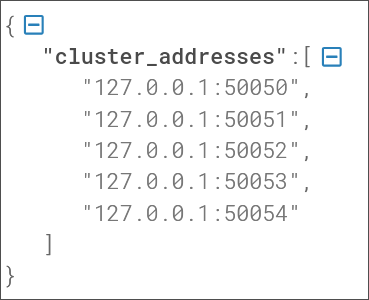
\includegraphics[scale=0.4]{inc/client-config.png}
  \caption{Пример клиентского конфигурационного файла}
  \label{fig:client_config}
\end{figure}

Клиент инициализирует пул соединений к указанным адресам и выбирает рабочую
«точку входа» по порядку (или по доступности). При ошибке соединения
выполняется следующий адрес из списка, что обеспечивает толерантность к отказу
отдельного узла без участия пользователя. Запросы, изменяющие состояние
(постановка задачи), отправляются на любой доступный узел; при необходимости
выполняется прозрачный редирект на лидера.

Второй файл задаёт путь для сохранения результатов и имя динамической
библиотеки задачи (см. рис.~\ref{fig:user_config})

\begin{figure}
  \centering
  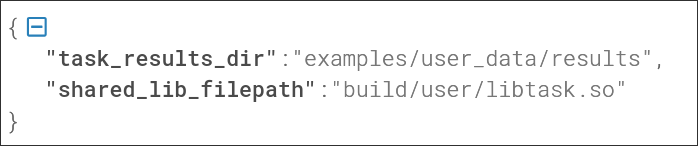
\includegraphics[scale=0.4]{inc/user-config.png}
  \caption{Пример пользовательского конфигурационного файла}
  \label{fig:user_config}
\end{figure}

Третий же файл содержит данные для задания (см. рис.~\ref{fig:user_data}).

\begin{figure}
  \centering
  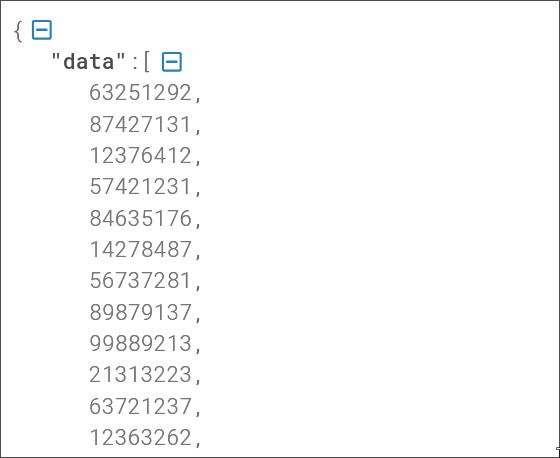
\includegraphics[scale=0.4]{inc/user-data.png}
  \caption{Пример данных для задания}
  \label{fig:user_data}
\end{figure}

\subsubsection{Протокол клиентского приложения}

Взаимодействие клиента с кластером реализовано поверх двунаправленного
потокового вызова \texttt{UserService.Connect}, определённого в gRPC (см. рис
~\ref{fig:user_proto}. Использование потокового RPC позволяет поддерживать
длительное соединение, через которое клиент и сервер обмениваются сообщениями в
обоих направлениях: клиент отправляет последовательность запросов, а сервер —
последовательность ответов, не прерывая сессию. Такой подход позволяет
объединить обнаружение лидера, постановку задачи и получение результата в
единый непрерывный диалог.

\begin{figure}
  \centering
  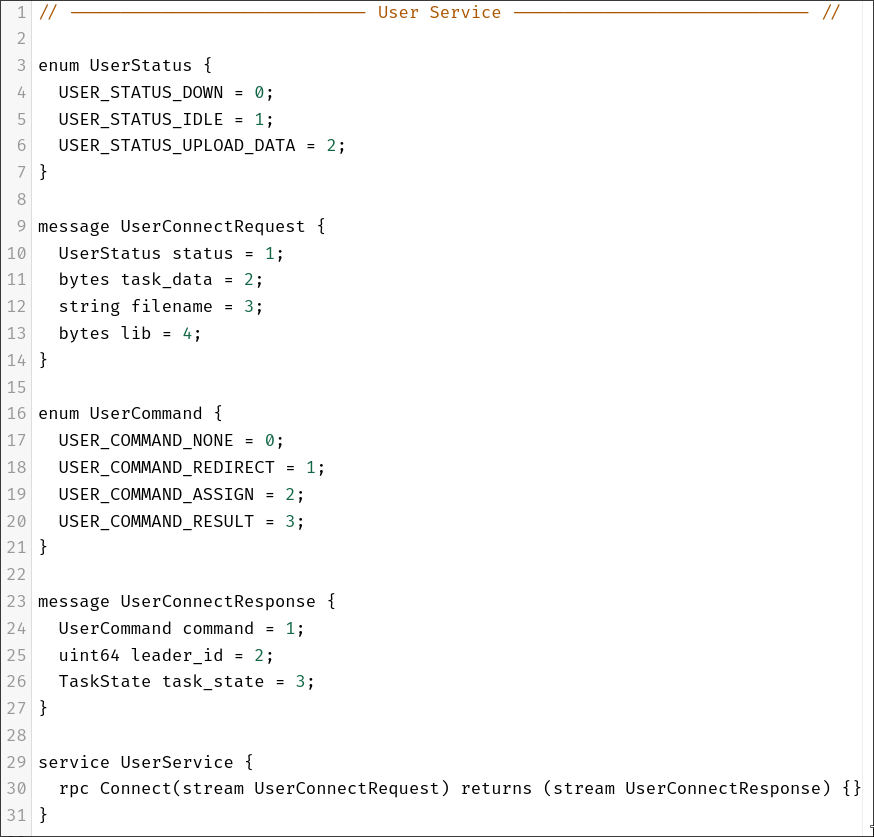
\includegraphics[scale=0.4]{inc/user-proto.png}
  \caption{Протокол общения клиента с кластером Raft}
  \label{fig:user_proto}
\end{figure}

Каждое сообщение клиента содержит поле \texttt{status}, отражающее фазу работы.
На этапе инициализации клиент посылает кадр со статусом \texttt{IDLE},
сигнализируя о готовности к работе. Если узел, на который был направлен запрос,
не является лидером кластера, сервер возвращает ответ с командой \texttt{REDIRECT}
и идентификатором актуального лидера. Получив такую команду, клиент закрывает
поток и устанавливает соединение с указанным узлом, гарантируя, что все
последующие запросы пойдут через единственный согласованный канал.

После установления соединения с лидером клиент переходит к передаче данных
задачи. Для этого используется статус \texttt{UPLOAD\_DATA}, а в сообщении
указываются полезная нагрузка (например, содержимое входного файла),
логическое имя этой нагрузки и идентификатор динамической библиотеки, которая
будет использована при выполнении задачи. Следует подчеркнуть, что по сети
передаётся только имя библиотеки, а не её бинарный образ, поскольку сами
модули заранее развёрнуты на вычислительных узлах. Сервер принимает эти данные,
реплицирует соответствующую команду в Raft-лог, а после достижения кворума
отправляет клиенту ответ с командой \texttt{ASSIGN}, в котором содержится
сгенерированный идентификатор задачи и подтверждение того, что она принята
кластером.

Соединение не разрывается после постановки задачи, а остаётся открытым до
получения финального результата. Когда задача завершается на воркере, её
результат реплицируется через Raft и фиксируется в машине состояний. Лишь
после этого сервер отправляет клиенту команду \texttt{RESULT}, содержащую
окончательный статус выполнения и, при необходимости, сериализованный результат.
Таким образом, клиент всегда получает согласованное состояние, подтверждённое
кворумом узлов.

В совокупности такой протокол обеспечивает упорядоченный и надёжный обмен:
постановка задачи и выдача результата проходят через единую двунаправленную
сессию, которая переносит всю сложность работы с распределённым кластером на
серверную сторону. Клиенту не требуется отслеживать состояние выборов или
дублировать запросы вручную: редиректы, подтверждения и уведомления о результате
получаются автоматически, что делает взаимодействие простым, но при этом
линейризуемым и устойчивым к сбоям.

\subsection{Реализация вычислительного узла}

Вычислительный узел (worker) предназначен для исполнения задач, поступающих из
кластера, и построен вокруг длительного двунаправленного потокового соединения
\texttt{WorkerService.Connect}. При запуске узел считывает локальную
конфигурацию, в которой указывается каталог для размещения динамических
библиотек (\texttt{libs\_dir}) (пример конфигурации приведен на
рис.~\ref{fig:worker_config}). Этот каталог используется как единое хранилище
исполняемых модулей, на которые ссылаются задания. Клиентская часть передаёт
библиотеку в кластер Raft; после репликации и коммита серверная сторона
распределённой системы доставляет содержимое соответствующего артефакта на
вычислительные узлы, где он сохраняется в \texttt{libs\_dir} и становится
доступным среде исполнения.

\begin{figure}
  \centering
  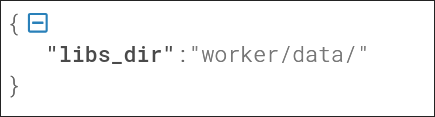
\includegraphics[scale=0.4]{inc/worker-config.png}
  \caption{Пример конфигурационного файла вычислительного узла}
  \label{fig:worker_config}
\end{figure}

Протокол общения вычислительного узла с кластером представлен на
рис.~\ref{fig:worker_proto}.

\begin{figure}
  \centering
  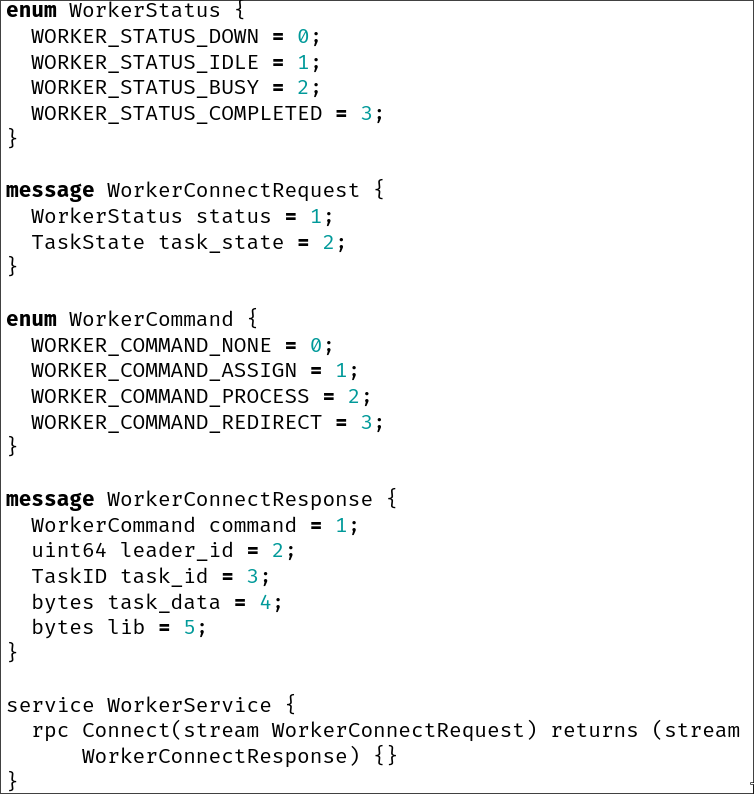
\includegraphics[scale=0.4]{inc/worker-proto.png}
  \caption{Протокол общения вычислительного узла с кластером Raft}
  \label{fig:worker_proto}
\end{figure}

Логика взаимодействия с кластером организована как непрерывная сессия. Сразу
после установления соединения вычислительный узел отправляет кадр с собственным
состоянием \texttt{IDLE}, тем самым сигнализируя о готовности к приёму работы.
Если подключение установлено не с лидером, сервер немедленно возвращает команду
перенаправления с указанием \texttt{leader\_id}; воркер закрывает текущий поток
и повторяет подключение к лидеру, после чего цикл продолжается без участия
оператора. В штатном режиме лидирующий сервер выдаёт команду назначения, в
которой указывает идентификатор задачи и, при необходимости, содержит полезную
нагрузку и бинарные данные библиотеки. В момент получения такого ответа воркер
выполняет атомарную подготовку окружения: проверяет наличие требуемого модуля в
\texttt{libs\_dir}, при отсутствии записывает поступивший образ на диск и
синхронно fsync’ит его, формируя детерминированное имя файла (например, по хешу
содержимого или по имени, пришедшему от сервера), после чего сверяет права
доступа и готовность к загрузке. Этим достигается инвариант, согласно которому
перед запуском пользовательского кода соответствующая библиотека обязательно
присутствует локально и доступна для динамического связывания.

Переход от состояния ожидания к выполнению инициируется командой
\texttt{PROCESS}. Получив её, узел запускает изолированный дочерний процесс
исполняющей среды (в проекте такой процесс может создаваться простым
\texttt{fork()} без сложной контейнеризации), загружает динамическую библиотеку
из \texttt{libs\_dir} и вызывает заранее оговорённый символ интерфейса,
передавая входные данные из \texttt{task\_data}. Основная служба воркера при
этом остаётся в состоянии «занят» и периодически отправляет в поток
\texttt{WorkerConnectRequest} собственный статус и актуальную проекцию
\texttt{TaskState}, обеспечивая наблюдаемость прогресса. В случае штатного
завершения исполняющий процесс формирует результат и отдаёт его основному
процессу узла; далее результат включается в \texttt{TaskState} и возвращается в
кластер тем же потоковым соединением. После этого вычислительный узел переводит
себя в состояние \texttt{COMPLETED}, что служит для серверной стороны сигналом
о готовности зафиксировать завершение в реплицированной машине состояний и
инициировать доставку результата клиенту.

Особое внимание уделено устойчивости к частичным сбоям. Если в ходе выполнения
падает дочерний процесс или попытка динамической загрузки модуля завершается
ошибкой, основная служба не теряет связь с кластером: воркер немедленно
фиксирует ошибочное завершение в \texttt{TaskState} и отправляет его через
активный поток, после чего возвращается в состояние \texttt{IDLE}. Повторы
команд со стороны сервера не приводят к дублированию работы: задача
идентифицируется по \texttt{task\_id}, поэтому воркер либо игнорирует повторные
\texttt{PROCESS} для уже завершённой задачи, либо корректно восстанавливает
исполнение, если сбой произошёл до выдачи финального состояния. Аналогично
сетевые разрывы и смена лидера обрабатываются на транспортном уровне: поток
может быть закрыт с соответствующим статусом gRPC, после чего узел повторяет
подключение с публикацией своего фактического состояния, а серверная сторона,
опираясь на зафиксированные в Raft переходы, восстанавливает согласованную
картину происходящего.

Таким образом, вычислительный узел реализует минимально необходимую
инфраструктуру для безопасного исполнения пользовательского кода: чтение
конфигурации и подготовка каталога библиотек; устойчивое потоковое соединение с
лидером кластера; детерминированная подготовка исполняемого окружения и
загрузка модулей из \texttt{libs\_dir}; изоляция пользовательского исполнения в
отдельном процессе; регулярная публикация статуса и финализация результата
через \texttt{WorkerService.Connect}. Все переходы по состояниям воркера
(\texttt{IDLE} $\rightarrow$ \texttt{BUSY} $\rightarrow$ \texttt{COMPLETED})
отражаются в потоке запросов, а сервер отвечает соответствующими командами
управления и данными (\texttt{ASSIGN}, \texttt{PROCESS}, \texttt{REDIRECT}),
сохраняя линейризуемую семантику наблюдения и единый порядок событий для всех
участников системы.

    \section{Ручное тестирование системы}

\subsection{Тестирование отказоустойчивости}

Проверка корректности реализации алгоритма Raft проводилась с использованием
ручных интеграционных испытаний. Для этого на локальной машине было запущено
три экземпляра Raft-узлов, каждый из которых инициализировался собственной
конфигурацией и прослушивал уникальный TCP-порт. На этапе инициализации узлы
формируют сетевые потоки (\texttt{peer threads}), регистрируют gRPC-сервисы и
начинают обмен heartbeat-сообщениями.

В первом эксперименте система демонстрирует штатное избрание лидера:
через заданный таймаут по истечении срока аренды один из узлов инициировал
выборы (лог содержит сообщение \texttt{Starting election in term 1}) и,
получив кворум голосов, объявил себя лидером (\texttt{I'm the leader now}).
В таком состоянии кластер готов принимать клиентские запросы, а
закоммиченные записи будут реплицироваться на оставшиеся узлы. Лог мастера
изображен на рис.~\ref{fig:leader_log}. Лог одной из реплик же представлен
на рис.~\ref{fig:replica_log}.

\begin{figure}
  \centering
  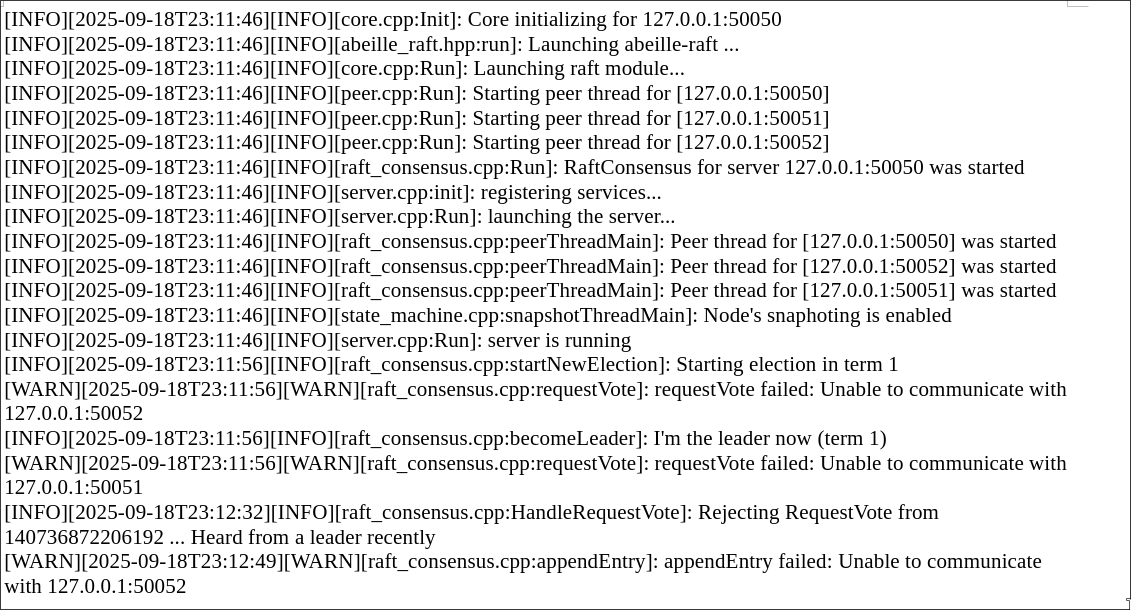
\includegraphics[scale=0.4]{inc/leader-log.png}
  \caption{Лог мастера при первом выборе лидера}
  \label{fig:leader_log}
\end{figure}

\begin{figure}
  \centering
  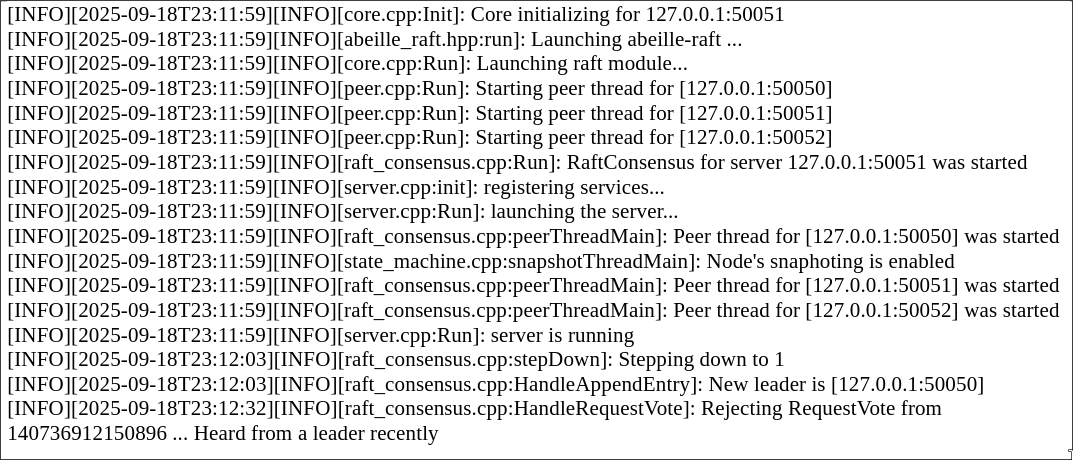
\includegraphics[scale=0.4]{inc/replica-log.png}
  \caption{Лог реплики при первом выборе лидера}
  \label{fig:replica_log}
\end{figure}

Затем моделировался отказ лидера: первый узел был остановлен, что привело к
прекращению рассылки heartbeat-пакетов (см. рис.~\ref{fig:leader-shutdown}).

\begin{figure}
  \centering
  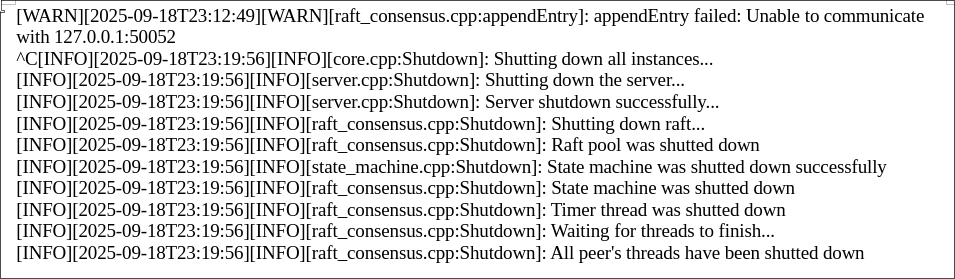
\includegraphics[scale=0.4]{inc/master-after-shutdown.png}
  \caption{Логи при остановке мастера}
  \label{fig:leader-shutdown}
\end{figure}

Спустя период \texttt{election timeout} один из оставшихся узлов инициировал
новый раунд выборов (терм 2), получил поддержку большинства и стал новым
лидером. В логах зафиксировано событие \texttt{becomeLeader} с указанием нового
терма, что подтверждает корректную работу механизма смены лидерства и
сохранение согласованности состояния кластера, это представлено на рис.
~\ref{fig:new-master}.

\begin{figure}
  \centering
  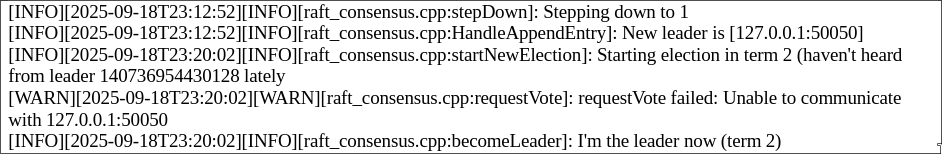
\includegraphics[scale=0.4]{inc/replica-master-after-shutdown.png}
  \caption{Логи нового мастера после остановки старого}
  \label{fig:new-master}
\end{figure}

Процесс голосования реплики за нового лидера представлен на рис.
~\ref{fig:replica-after-new-leader}.

\begin{figure}
  \centering
  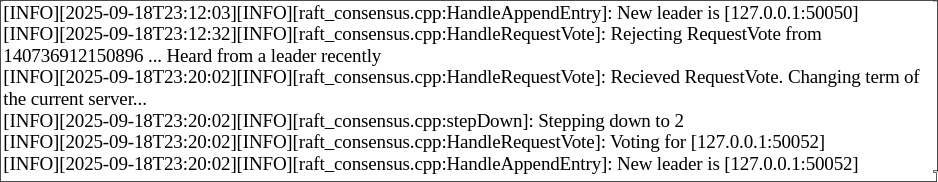
\includegraphics[scale=0.4]{inc/replica-after-shutdown.png}
  \caption{Процесс голосования за нового лидера}
  \label{fig:replica-after-new-leader}
\end{figure}

Такие испытания позволяют убедиться, что система корректно реагирует на сбои:
потеря лидера не приводит к недоступности сервиса, а лишь инициирует повторные
выборы, после которых кластер восстанавливает способность обрабатывать запросы.
В сочетании с механикой репликации и commit-индексов это гарантирует, что все
закоммиченные записи остаются видимыми для клиента даже при перезапуске узлов.

\subsection{Инициализация клиентского приложения и подключение к кластеру}

Тестирование вычислительного процесса начинается с запуска консольного клиента
с указанием конфигурационных файлов пользователя и кластера. На
рис.~\ref{fig:client_start} приведён фрагмент журнала запуска клиента. В ходе
подключения клиент последовательно обходит адреса, указанные в
\texttt{client\_config.json}. Поскольку первый узел кластера
(\texttt{127.0.0.1:50050}) в момент запуска был недоступен, попытка
установления соединения завершилась ошибкой, что зафиксировано в логах с
уровнем \texttt{ERROR}. После истечения интервала переподключения клиент
автоматически переходит к следующему адресу и успешно устанавливает соединение
с узлом \texttt{127.0.0.1:50051}, а затем и с \texttt{127.0.0.1:50052}. Такая
стратегия повышает отказоустойчивость системы: пользователь не обязан вручную
выбирать рабочий узел, так как клиент сам находит доступного участника
кластера.

\begin{figure}[h!]
    \centering
    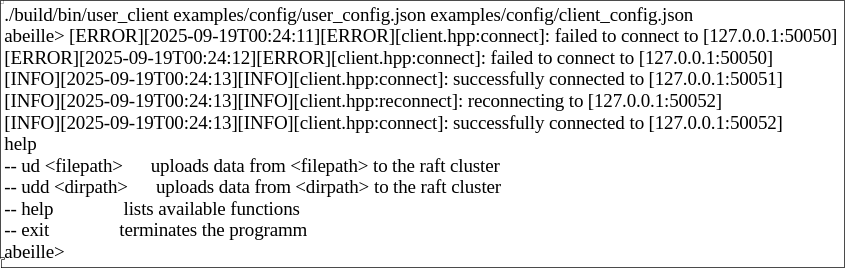
\includegraphics[width=0.8\linewidth]{inc/client-shell.png}
    \caption{Журнал запуска клиентского приложения: обработка недоступности узла и
    успешное подключение к кластеру.}
    \label{fig:client_start}
\end{figure}

После установления соединения клиент переходит в интерактивный режим, предлагая
пользователю список доступных команд. В частности, доступны функции загрузки
данных из файла или директории (\texttt{ud}, \texttt{udd}), вывод справочной
информации и завершение работы программы. На этом этапе система готова к
приёму задания и дальнейшему тестированию логики репликации и обработки задач.

\subsection{Запуск вычислительных узлов и их подключение к кластеру}

После инициализации клиентской части производится запуск вычислительных узлов,
которые будут непосредственно выполнять задачи.Логи на
рис.~\ref{fig:worker_start} демонстрируют, что, как и в случае с клиентом,
воркер поочерёдно пытается подключиться к указанным в
\texttt{client\_config.json} узлам. Первая пара попыток к
\texttt{127.0.0.1:50050} завершилась ошибкой соединения, после чего воркер
переключился на следующий адрес и успешно установил потоковое RPC-соединение с
\texttt{127.0.0.1:50051}, а затем и с лидером \texttt{127.0.0.1:50052}.

\begin{figure}[h!]
    \centering
    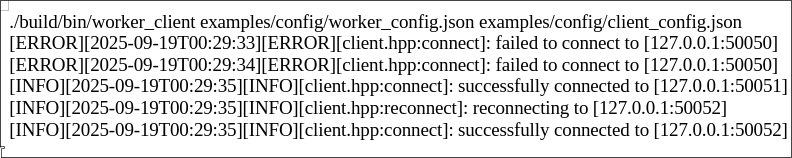
\includegraphics[width=0.8\linewidth]{inc/worker-log.png}
    \caption{Логи запуска вычислительного узла: автоматический обход узлов и успешное подключение.}
    \label{fig:worker_start}
\end{figure}

После установления соединения воркер переходит в состояние \texttt{IDLE},
публикуя свой статус в поток \texttt{WorkerService.Connect}, что позволяет
кластеру учитывать его при назначении новых задач. Таким образом, уже на этом
этапе проверяется важная функциональность системы — автоматический выбор
доступного узла и готовность воркера принимать задания от лидера кластера.

\subsection{Тестирование выполнения задания}

Для проверки корректности работы системы был проведён end-to-end тест с
использованием простого вычислительного задания. В качестве тестовой функции
был выбран алгоритм факторизации числа на простые множители, реализованный на
C++. Такая задача является хорошим примером для функционального тестирования:
она не требует сложной подготовки данных, но даёт детерминированный и легко
проверяемый результат. Код задания представлен в приложении В. В качестве
входных данных подавались 10000 чисел.

Постановка задачи выполнялась из интерактивной консоли клиентского приложения с
помощью команды \texttt{ud}, передающей содержимое \texttt{data.json} в
кластер. Это представлено на рис.~\ref{fig:client-send}. Клиент подтвердил
успешную загрузку данных, а после обработки задачи вывел сообщение о получении
результата.

\begin{figure}[h!]
    \centering
    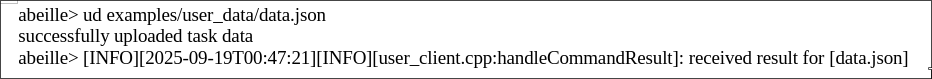
\includegraphics[width=0.8\linewidth]{inc/client-send.png}
    \caption{Процесс пересылки данных на клиенте}
    \label{fig:client-send}
\end{figure}

На стороне лидера Raft логи показан полный путь задачи: назначение её
конкретному воркеру, репликацию соответствующей команды в Raft-лог, достижение
кворума и коммит, а также последующую фиксацию результата (см.
рис.~\ref{fig:master-log-task}). При этом реплика синхронизировалась с лидером,
что видно по сообщениям \texttt{HandleAppendEntry} и обновлению индексов
коммита (см. рис.~\ref{fig:replica-log-task}).

\begin{figure}[h!]
    \centering
    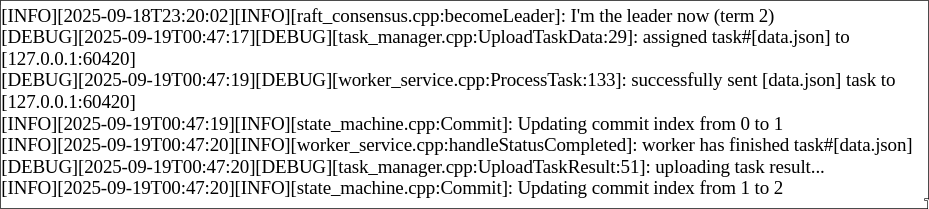
\includegraphics[width=0.8\linewidth]{inc/master-log-task.png}
    \caption{Лог мастера при назначении задания}
    \label{fig:master-log-task}
\end{figure}

\begin{figure}[h!]
    \centering
    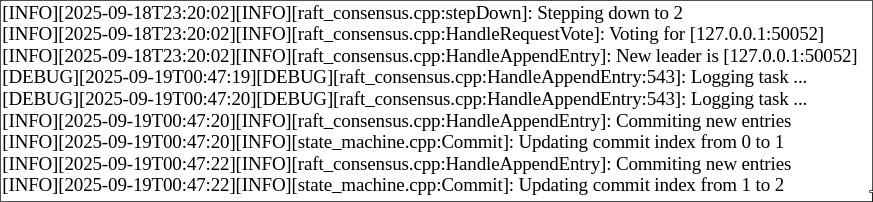
\includegraphics[width=0.8\linewidth]{inc/replica-log-task.png}
    \caption{Лог реплики при назначении задания}
    \label{fig:replica-log-task}
\end{figure}

Логи вычислительного узла подтвердили успешное получение задания: воркер перешёл
в состояние \texttt{BUSY}, инициировал локальный процесс обработки данных
через IPC, корректно завершил вычисление и вернул результат обратно в кластер
(см. рис.~\ref{fig:worker-log-task}).

\begin{figure}[h!]
    \centering
    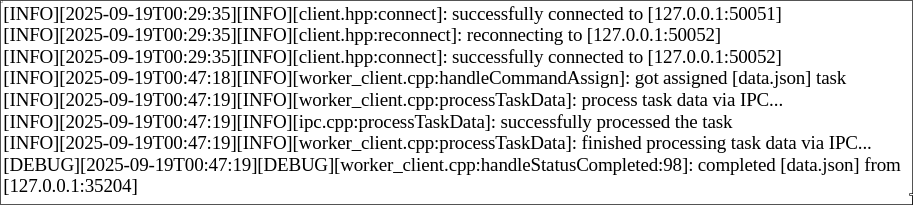
\includegraphics[width=0.8\linewidth]{inc/worker-log-task.png}
    \caption{Лог вычислительного узла при выполнении работы}
    \label{fig:worker-log-task}
\end{figure}

На стороне мастера была зафиксирована команда \texttt{RAFT\_COMMAND\_MOVE},
переведшая задачу в статус завершённой, после чего результат был передан
пользовательскому клиенту. Таким образом, в рамках теста была проверена вся
цепочка обработки: от приёма входных данных до финализации состояния в машине
состояний и возврата результата.

Проведённый эксперимент подтверждает корректность реализации основных
механизмов системы: клиентские запросы реплицируются и коммитятся только при
достижении кворума, воркеры получают задачи и публикуют статус их выполнения,
а пользователь всегда наблюдает согласованное состояние кластера, даже при
ранее проведённых сменах лидера или мертвых узлах.

\subsection{Нагрузочный тест с 50 параллельными клиентами}

Для проверки поведения системы при высокой конкурентной нагрузке был
организован сценарий с одновременной работой пятидесяти клиентских процессов.
Каждый клиент открывал двунаправленное gRPC-соединение с кластером, отправлял
одну команду \texttt{ud} для постановки задачи в очередь и завершал работу,
освобождая слот для следующих запусков. Параллельный запуск был реализован
средствами утилиты \texttt{GNU parallel} (см. рис.~\ref{fig:leader-multi-conn}),
обеспечивающей одновременный запуск 50 процессов с минимальной задержкой между
стартами.

\begin{figure}[h!]
    \centering
    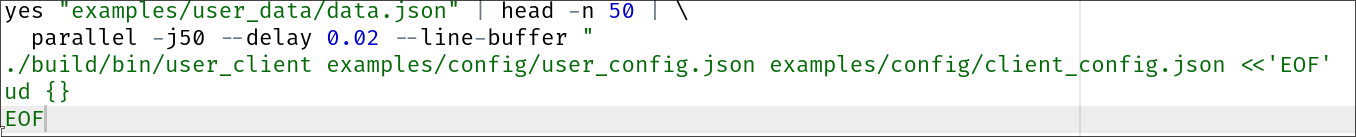
\includegraphics[width=0.95\linewidth]{inc/load-multi.png}
    \caption{Нагрузочный тест}
    \label{fig:leader-multi-conn}
\end{figure}

В данном тесте использовались два рабочих узла (воркера). Кластер Raft выбрал
лидера в начале прогона, после чего последовательно обрабатывал поступающие
задания. В журнале лидера наблюдается монотонное увеличение индекса коммита
каждой новой записи лога (рис.~\ref{fig:leader_log_50}), что подтверждает
корректную репликацию команд и достижение кворума. Каждое успешно завершённое
задание сопровождается сообщением
\texttt{worker\_service.cpp:handleStatusCompleted}, после чего в машине
состояний фиксируется переход задачи из состояния \texttt{assigned} в
\texttt{completed}.

\begin{figure}[h!]
    \centering
    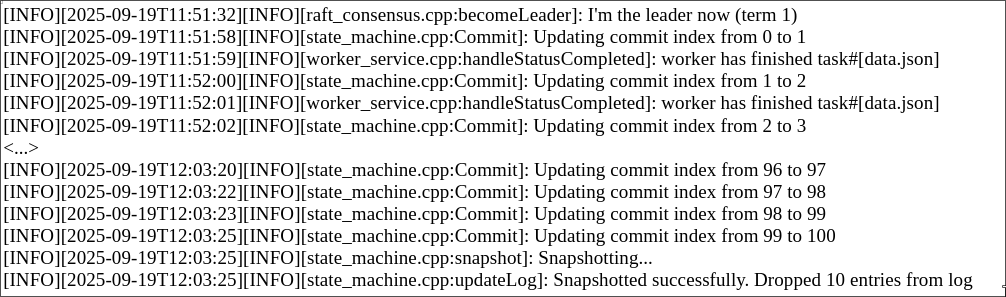
\includegraphics[width=0.95\linewidth]{inc/leader-multi-conn.png}
    \caption{Фрагмент лога лидера во время нагрузочного теста с 50 клиентами}
    \label{fig:leader_log_50}
\end{figure}

При достижении сотого коммита сработал механизм создания снепшота, что
подтверждается сообщением \texttt{Snapshotting...} в логах. После успешного
сохранения состояния машины состояний на диск (\texttt{Snapshotted
successfully}) из лога были удалены 10 записей, как и предусмотрено параметром
\texttt{snapshot\_after} в конфигурации. Продолжение работы кластера после
создания снепшота не вызвало увеличения задержек или ошибок репликации, что
свидетельствует о корректности реализации механизма архивации и его
прозрачности для клиентских приложений.

Таким образом, тест показал, что система способна обрабатывать десятки
одновременных подключений, сохраняя линейризуемость состояния и выполняя
своевременное архивирование лога без нарушения доступности сервиса.

\subsection{Тестирование на задаче с большим объёмом данных}

Для проверки корректности работы системы при выполнении ресурсоёмких задач был
проведён эксперимент с входными данными увеличенного размера (около двух
миллионов элементов). Задача была отправлена в кластер с использованием
стандартного клиента и поступила на один из доступных рабочих узлов. Фрагмент
лога воркера приведён на рис.~\ref{fig:worker_bigdata}.

\begin{figure}[h!]
    \centering
    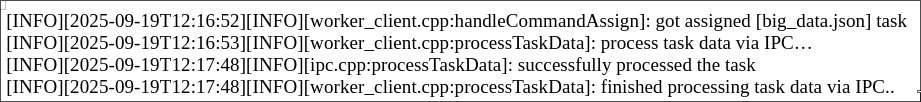
\includegraphics[width=0.95\linewidth]{inc/worker-big-data.png}
    \caption{Лог вычислительного узла при обработке задачи с 2 млн элементов}
    \label{fig:worker_bigdata}
\end{figure}

Как видно из лога, узел получил команду назначения задачи
(\texttt{handleCommandAssign}), после чего перешёл к фазе обработки данных через
IPC-механизм (\texttt{processTaskData}). Общая длительность обработки составила
около 56 секунд, что соответствует ожидаемому времени выполнения для задачи
данного объёма. По завершении вычислений задача была успешно отмечена как
выполненная (\texttt{finished processing task data via IPC}), а результат был
передан обратно в кластер и зафиксирован в машине состояний.

Данный эксперимент подтвердил, что система корректно обрабатывает задачи
увеличенной сложности и объёма, при этом не теряя связи с кластером и
сохраняя линейризуемость состояния. В течение всего времени выполнения других
ошибок или повторных назначений задачи не наблюдалось, что демонстрирует
устойчивость и надёжность реализации даже при продолжительных вычислениях.


    \conclusion

В ходе прохождения практики был проведён комплексный анализ механизма
шардирования в СУБД Tarantool. Основное внимание было уделено изучению
архитектуры модуля \texttt{vshard}, принципов распределения данных и
обеспечения согласованности при выполнении операций в шардированном кластере.

Были рассмотрены и проанализированы существующие подходы к реализации
Map-Reduce запросов по репликам. В результате исследования выявлены ключевые
проблемы, связанные с обеспечением консистентности данных при выполнении
распределённых запросов, и предложена альтернативная реализация.

Практическая значимость работы заключается в:
\begin{itemize}
    \item Систематизации знаний о работе шардированного кластера Tarantool;
    \item Выявлении ограничений существующей реализации модуля \texttt{vshard};
    \item Разработке предложений по расширению функциональности для поддержки
        Map-Reduce операций по репликам.
\end{itemize}

Полученные результаты могут быть использованы для дальнейшего развития модуля
шардирования Tarantool и улучшения его безопасности. Проведённое исследование
демонстрирует важность комплексного подхода к проектированию распределённых
систем и необходимость тщательного анализа требований к согласованности данных.

Результаты работы подтверждают возможность реализации эффективного механизма
выполнения Map-Reduce запросов по репликам в шардированной среде с соблюдением
требований к консистентности данных и производительности системы.


    \printbibliography

    \appendix
    \appendixsection{Основы теории решёток}

В последние годы решётки служат алгоритмическим инструментом для решения
широкого круга задач в информатике, математике и криптографии, особенно в
квантовоустойчивых криптографических протоколах. Ниже приведены базовые понятия
и известные алгоритмы, тесно связанные с нашей работой.

\subsection*{Базовые понятия}

Пусть $\lVert\cdot\rVert$ — евклидова норма векторов из $R^{m}$. Векторы
отмечаем полужирным (в переводе этого нет), матрицы пишем построчно; элементы
матрицы $M$ обозначаем $m_{i,j}$. Верхний индекс~$T$ — транспонирование.

\begin{itemize}
\item \textbf{Решётка.} Пусть $b_{1},\ldots,b_{n}\in R^{m}$ — линейно
        независимые столбцы, тогда множество всех линейных комбинаций их
        целочисленных коэффициентов — решётка, определяемая как
        \begin{equation} \Lambda(B) =\{\,Bx \mid x\in Z^{n}\,\} =\{\,b =
            x_{1}b_{1}+\dots+x_{n}b_{n} \mid x_{1},\dots,x_{n}\in Z\,\}.
        \end{equation} где $B=[b_{1},\ldots,b_{n}]\in R^{m\times n}$ — матрица
        базиса, которая также может быть использована чтобы представлять
        решетку для простоты. $\{b_1, \ldots, b_n\}$ - группа базиса решетки.
        Размерность решётки $n$. Её детерминант $\det\Lambda=(\det
        B^{T}B)^{1/2}$, здесь $B^T$ - транспонированная матрица $B$. При
        квадратной $B$ имеем $\det\Lambda=\det B$. Детерминант представляет
        объём решётки в геометрическом представлении, обозначается как
        $\operatorname{vol}(\Lambda)$. Длина точки $b\in R^{m}$ определяется
        как $\lVert b\rVert=(b^{T}b)^{1/2}$.

\item \textbf{Последовательные минимумы.} Для $n$‑мерной решётки $\Lambda$
        положительные числа $\lambda_{1}(\Lambda)\le\lambda_{2}(\Lambda)
        \le\dots\le\lambda_{n}(\Lambda)$ называются последовательными
        минимумами, где $\lambda_{k}(\Lambda)$ — наименьший радиус шара с
        центром в нуле, содержащего $k$ линейно независимых векторов из
        $\Lambda$. Обозначим $\lambda_{1}=\lambda_{1}(\Lambda)$ как длину
        кратчайшего ненулевого вектора из $\Lambda$.

\item \textbf{Постоянная Эрмита.} Эрмитовым инвариантом решётки $\Lambda$
        называется
        \begin{equation}
          \gamma(\Lambda)
          = \frac{\lambda_{1}^{2}(\Lambda)}{\operatorname{vol}(\Lambda)^{2/n}}
          = \frac{\lambda_{1}^{2}(\Lambda)}{\det(\Lambda)^{2/n}}.
        \end{equation}

        Постоянная Эрмита $\gamma_{n}$ — максимальное значение $\gamma(\Lambda)$
        для всех $n$‑мерных решёток, или минимальное константное $\gamma$,
        удовлетворяющее $\lambda_{1}(\Lambda)^{2}\le\gamma(\det\Lambda)^{2/n}$
        для всех решёток размености $n$ соответственно.

\item \textbf{QR‑разложение.} У решёточной матрицы базиса $B$ есть единственное
        разложение $B=QR\in R^{m\times n}$, где $Q\in R^{m\times n}$,
        $R=[r_{i,j}]_{1\le i,j\le n} \in R^{n\times n}$, здесь $Q\in R^{m\times
        n}$ — изомет­рическая (столбцы ортогональны и единичной длины), а $R
        \in R^{n\times n}$ — верхнетреугольная матрица с положительными
        диагональными элементами $r_{i,i}$. Коэффициенты Грама–Шмидта
        $\mu_{j,i}=r_{i,j}/r_{i,i}$ легко вычисляются из QR‑разложения. Для
        целочисленной $B$ коэффициенты $\mu_{j,i}$ обычно рациональны.

\item \textbf{Задача кратчайшего вектора (SVP).}
      Дана группа базиса $B$ решётки $\Lambda$.

      \begin{itemize}
          \item Задача кратчайшего вектора (SVP): Требуется найти вектор
              $v\in\Lambda$, такой что $\lVert v\rVert=\lambda_{1}(\Lambda)$.
          \item Приближённая задача кратчайшего вектора ($\alpha$‑SVP): Найти
              ненулевой вектор $v\in\Lambda$, удовлетворяющий
              $\lVert v\rVert\le\alpha\,\lambda_{1}(\Lambda)$.
          \item Эрмитова задача кратчайшего вектора ($r$‑Hermite SVP):
              Найти ненулевой вектор $v\in\Lambda$, такой что
              $\lVert v\rVert \;\le\; r\,\det(\Lambda)^{1/n}$.
      \end{itemize}

      Параметр $\alpha\ge1$ в $\alpha$‑SVP называется фактором аппроксимации.
      Обычнро задача упрощается при увеличении $\alpha$. При $\alpha=1$ задачи
      $\alpha$‑SVP и SVP совпадают. Истинное значение $\lambda_{1}$ в
      $\alpha$‑SVP трудно вычислить из-за сложности SVP, поэтому решение
      $\alpha$‑SVP не всегда легко проверить. Задача $r$‑Hermite SVP является
      вычислимой (относительно просто вычислимой), она определяется величиной
      $\det(\Lambda)^{1/n}$ вместо $\Lambda_1$. В результате, мы можем лешко
      проверить решение, но не можем сравнить его с кратчайшим вектором.

\item \textbf{Задача ближайшего вектора (CVP)}
      Дана группа базиса $B$ решётки $\Lambda$ и целевой вектор
      $t\in\operatorname{span}(B)$.

      \begin{itemize}
          \item Задача ближайшего вектора (CVP): Найти вектор $v\in\Lambda$,
              такой что расстояние $\lVert v - t\rVert$ может быть минимизировано,
              т.е. $\lVert v - t\rVert = \operatorname{dist}(\Lambda,t)$.
          \item $\alpha$-приближенная задача ближайшего вектора ($\alpha$‑CVP):
              Найти вектор $v\in\Lambda$, такой что расстояние
              $\lVert v - t\rVert \le \alpha \times \operatorname{dist}(\Lambda,t)$
          \item $r$-приближенная задача ближайшего вектора (($r$‑AbsCVP):  Найти
              $v\in\Lambda$ такое, что $\lVert v - t\rVert \le r$.
      \end{itemize}

      Определения аналогичны случаям для SVP; параметр $\alpha\ge1$ в
      $\alpha$‑CVP играет ту же роль, что и в $\alpha$‑SVP. В $r$‑AbsCVP
      параметр $r$ может быть любым разумным значением, соизмеримым с
      $\operatorname{dist}(\Lambda,t)$, например $\det(\Lambda)^{1/n}$ в
      $r$‑Hermite SVP.
\end{itemize}

\subsection*{Алгоритм LLL}
\begin{algorithm}[htp!]
    \SetAlgoLined

    \KwData{базис решётки $\text{b}_1, \dots, \text{b}_n \in \text{Z}^m$, параметр $\delta$}
    \KwResult{$\delta$-LLL-редуцированный базис}

    \textbf{Шаг 1:} Орторгонализация Грама-Шмидта \\
    Выполнить орторгонализацию Грама-Шмидта для базиса $\text{b}_1, \dots, \text{b}_n$, обозначим результат как $\tilde{\text{b}}_1, \dots, \tilde{\text{b}}_n \in \text{R}^m$

    \textbf{Шаг 2:} Редукция

    \For{$i = 2$; $i < n$; $i = i + 1$}{
        \For{$j = i-1$; $i > 1$; $ i = i - 1$}{
            $c_{i,j} = \left\lfloor \dfrac{\langle \text{b}_i, \tilde{\text{b}}_j \rangle}{\langle \tilde{\text{b}}_j, \tilde{\text{b}}_j \rangle} \right\rceil$; \\
            $\text{b}_i \gets \text{b}_i - c_{i,j} \cdot \text{b}_j$;
        }
    }

    \textbf{Шаг 3:} Обмен

    \If{$\exists \, i$ такое, что $\delta \cdot \| \tilde{\text{b}}_i \|^2 > \| \mu_{i+1,i} \tilde{\text{b}}_i + \tilde{\text{b}}_{i+1} \|^2$}{
        $\text{b}_i \leftrightarrow \text{b}_{i+1}$; \\
        перейти к шагу 1;
    }

    \textbf{Шаг 4:} Вывод базиса $\text{b}_1, \dots, \text{b}_n$

    \caption{Алгоритм LLL-редукции}
    \label{alg:lll}
\end{algorithm}

Алгоритм LLL — один из самых известных алгоритмов редукции решётки; он был
предложен А. К. Ленстрой, Х. В. Ленстрой (мл.) и Л. Ловашем в 1982 г.
\cite{cite_35}. Для $n$‑мерной решётки этот алгоритм позволяет решать $\alpha
\;=\; \left(\frac{2}{\sqrt{3}}\right)^{n}$ за полиномиальное время. Ниже
приведены связанные понятия и алгоритмы.

\newcounter{tmp-enum-lll}

\begin{itemize}
    \item \textbf{LLL базиc}: Базис $B = QR$ называется LLL‑редукции или
        LLL‑базисом при параметре редукции $\delta\in(1/4,1]$, если выполняются
        условия:
        \begin{enumerate}
            \item $\frac{\lvert r_{i,j}\rvert}{r_{i,i}} \;\le\; \frac12, \quad \text{for all } j > i;$
            \item $\delta\, r_{i,i}^{2}\;\le\;r_{i,i+1}^{2} + r_{i+1,i+1}^{2},\quad \text{for } i = 1,\ldots,n-1.$
            \setcounter{tmp-enum-lll}{\value{enumi}}
        \end{enumerate}

        Очевидно, LLL‑базис также удовлетворяет
        \( r_{i,i}^{2} \le \alpha\, r_{i+1,i+1}^{2} \),
        для \(\alpha = \frac{1}{(\delta - 1 / 4)}\).

        Параметры, рассматриваемые в оригинальной литературе по алгоритму LLL,
        равны $\delta = \tfrac34$, $\alpha = 2$. Известный результат о LLL‑базисе
        показывает, что для любого $\delta < 1$ LLL‑базис может быть получен за
        полиномиальное время и хорошо аппроксимирует последовательные минимумы\:

        \begin{enumerate}
            \setcounter{enumi}{\value{tmp-enum-lll}}
            \item $\alpha^{-\,i+1} \;\le\; \lVert b_{i}\rVert^{2}\,\lambda_{i}^{-2}
                \;\le\; \alpha^{\,n-1}, \quad \text{for } i = 1,\ldots,n;$
            \item $\lVert b_{1}\rVert^{2} \;\le\; \alpha^{\frac{n-1}{2}}\,
                \bigl(\det\Lambda\bigr)^{2/n}.$
        \end{enumerate}

    \item \textbf{Алгоритм LLL}: Для заданного набора базиса
        $B = [b_{1},\ldots,b_{n}] \in Z^{m\times n}$
        алгоритм может привести его к LLL‑редуцированному виду
        или преобразовать в LLL‑базис. Алгоритм состоит из трёх
        основных шагов: ортогонализация Грама–Шмидта, редукции и
        обмен. Конкретные шаги приведены в Алгоритме \ref{alg:lll}.
\end{itemize}

\subsection*{Алгоритм ближайшей плоскости Бабая}

Алгоритм ближайшей плоскости Бабая \cite{cite_32} (далее — алгоритм Бабая)
применяется для решения CVP. Для $n$‑мерной решётки он может получать фактор
аппроксимации $\alpha \;=\; 2\!\left(\frac{2}{\sqrt{3}}\right)^{n}$ для
$\alpha$‑CVP. Алгоритм состоит из двух этапов, первый из которых заключается в
редукции решетки с помощью алгоритма LLL. Второй является процедурой уменьшения
размера, который в основном вычисляет линейную комбинацию целочисленных
коэффициентов, ближайших к целевому вектору $t$ в LLL-базисе. Этот шаг по сути
совпадает со вторым шагом в LLL-редукции. Подробные действия приведены в
Алгоритме \ref{alg:babai}.

\begin{algorithm}[htp!]
    \SetAlgoLined

    \KwData{базис решётки $\text{b}_1, \dots, \text{b}_n \in \text{Z}^m$, параметр $\delta = 3/4$, целевой вектор $\text{t} \in \text{Z}^m$}
    \KwResult{вектор $\text{x} \in \Lambda(B)$, такой что $\|\text{x} - \text{t}\| \leq 2^{n/2} \, \text{dist}(\text{t}, \Lambda(B))$}

    \textbf{Шаг 1:} LLL-редукция \\
    Применить LLL-редукцию к базису $B$ с параметром $\delta$ \\
    Обозначим результат: $\tilde{\text{b}}_1, \dots, \tilde{\text{b}}_n \in \text{R}^m$

    \textbf{Шаг 2:} Уменьшение размера \\
    $\text{b} \gets \text{t}$

    \For{$j = n$; $j > 1$ $j = j-1$}{
        $c_j = \left\lfloor \dfrac{\langle \text{b}, \tilde{\text{b}}_j \rangle}{\langle \tilde{\text{b}}_j, \tilde{\text{b}}_j \rangle} \right\rceil$ \\
        $\text{b} \gets \text{b} - c_j \cdot \text{b}_j$
    }

    \textbf{Шаг 3:} Вернуть $\text{t} - \text{b}$

    \caption{Алгоритм Бабая}
    \label{alg:babai}
\end{algorithm}

    \appendixsection{Алгоритм Шнорра для факторизации целых чисел}

\subsection*{Метод решета Шнорра}

Рассмотрим общую задачу факторизации, в которой задано целое число $N$,
предполагается разложить его на два нетривиальных множителя $p<q$, так что $N =
p\times q$. Метод решета для факторизации начинается с определения пары гладких
отношений.

Пусть $p_i,\; i = 1,\dots,n$ — первые $n$ простых чисел вместе с $p_0$,
удовлетворяющими $-1 = p_0 < 1 < p_1 < \dots < p_n < p$. Множество $P =
\{p_i\}_{i=0,\dots,n}$ называется простым базисом. Число $p_0 = -1$ не является
простым, однако включается для учёта знака целого числа. Целое число называется
$p_n$‑гладким, если все его простые делители меньше $p_n$; число $p_n$ при этом
называют пределом гладкости. Пара целых чисел $(u_j,v_j)$ называется
$p_n$‑гладкой парой, если и $u_j$, и $v_j$ являются $p_n$‑гладкими. Более того,
пара целых чисел $(u_j,v_j)$ называется $p_n$‑гладкой парой отношений
(сокращённо sr‑пара), если:

\begin{equation}
  u_{j} \;=\; \prod_{i=1}^{n} p_{i}^{\,e_{i,j}},
  \qquad
  u_{j} - v_{j}N \;=\; \prod_{i=0}^{n} p_{i}^{\,e'_{i,j}},
\end{equation}

\noindent где $e_{i,j},\,e'_{i,j}\in{N}$, тогда имеем

\begin{equation}
  \frac{u_{j}-v_{j}N}{u_{j}}
  \;\equiv\;
  \prod_{i=0}^{n} p_{i}^{\,e'_{i,j}-e_{i,j}}
  \;\equiv\; 1 \pmod{N}.
\end{equation}

Следует отметить, что гладкая пара отличается от sr‑пары: sr‑пара должна не
только быть $p_n$‑гладкой, но и удовлетворять более строгим условиям в
уравнении Б.3. Пусть $S=\{(u_j,v_j)\}_{j=1,\dots,n+1}$ — набор из $n\!+\!1$
sr‑пар. Пусть существуют коэффициенты $ t_1,\dots,t_{n+1}\in\{0,1\}$, такие что:

\begin{equation}
  \sum_{j=1}^{n+1} t_{j}\bigl(e'_{i,j}-e_{i,j}\bigr)
  \;\equiv\; 0 \pmod{2},
  \qquad i = 0,1,\dots,n.
\end{equation}

\noindent Обозначим $X \;=\ \prod_{i=0}^{n}p_{i}^{\frac12 \sum_{j=1}^{n+1} t_{j}\bigl(e'_{i,j}-e_{i,j}\bigr)},$
тогда

\begin{equation}
  X^{2}-1 \;=\; (X+1)(X-1) \;\equiv\; 0 \pmod{N}.
\end{equation}

\noindent Если $X \not\equiv \pm1 \pmod{N}$, то нетривиальный фактор числа $N$
получается как $\gcd(X \pm 1,\, N)$.

Поскольку размерность системы линейных уравнений равна~$O(n)$ и она решается
за~$O(n^{3})$ операций, эту малую часть вычислений при факторизации~$N$ мы
опускаем. Следовательно, задача факторизации сводится к задаче поиска sr‑пары.
В дальнейшем эта задача будет преобразована в задачу ближайшего вектора на
решётке.

\subsection*{Построение решётки и целевого вектора}

sr‑пары будут получены из приближённого решения задачи CVP в алгоритме Шнорра.
Сначала опишем построение простой решётки $\Lambda(B_{n,c})$ и целевого вектора
$t\in \mathbb{R}^{\,n+1}$; здесь $c>0$ — настраиваемый параметр. Матрица решётки
$B_{n,c}=[b_{1},\dots,b_{n}]\in \mathbb{R}^{(n+1)\times n}$ задаётся

\begin{equation}
  B_{n,c} =
  \begin{pmatrix}
    f(1)      & 0        & \dots & 0        \\
    0         & f(2)     & \dots & 0        \\
    \vdots    & \vdots   & \ddots& \vdots   \\
    0         & 0        & \dots & f(n)     \\
    N^{c}\ln p_{1} & N^{c}\ln p_{2} & \dots & N^{c}\ln p_{n}
  \end{pmatrix},
  \qquad
  t =
  \begin{pmatrix}
    0 \\[2pt]
    \vdots \\[2pt]
    0 \\[2pt]
    N^{c}\ln N
  \end{pmatrix}.
\end{equation}

\noindent где функции $f(i)$ при $i=1,\dots,n$ — случайные перестановки
диагональных элементов $(\sqrt{\ln p_{1}},\sqrt{\ln p_{2}},\dots, \sqrt{\ln
p_{n}})$.

Точку решётки или вектор можно представить целочисленной комбинацией базиса
решетки: $b=\sum_{i=1}^{n} e_{i} b_{i}\in\Lambda(B_{n,c})$, причём $e_{i}\in
Z$. Далее будем полагать, что $(u,v)$ — $p_{n}$‑гладкая пара и $\gcd(u,v)=1$.
Тогда $u,v$ выражаются через произведение простых чисел из простого базиса:

\begin{equation}
  u \;=\; \prod_{e_{i}>0} p_{i}^{\,e_{i}},
  \qquad
  v \;=\; \prod_{e_{i}<0} p_{i}^{\,-e_{i}}.
\end{equation}

В таком представлении гладкой паре $(u,v)$ взаимно однозначно соответствует
вектор $b=(e_{1},\dots,e_{n})$ на решётке, пишем $b\sim(u,v)$. Таким образом,
вектор решётки кодирует гладкую пару.

Задача ближайшего вектора (CVP) формулируется как поиск вектора
$b_{0}\in\Lambda(B_{n,c})$, минимально удалённого от $t$:

\begin{equation}
    b_{0} \;=\; \arg\min_{\,b\in\Lambda}\;\lVert b - t\rVert.
\end{equation}

Согласно приведённому выше определению справедливо отношение:

\begin{equation}
  \lVert b - t\rVert^{2}
  \;\ge\;
  \ln(uv) \;+\; N^{2c}\,\bigl|\ln\tfrac{u}{vN}\bigr|^{2}.
\end{equation}

Уравнение выполняется тогда и только тогда, когда $e_{i}\in\{-1,0,1\}$, то есть
$u,v$ не содержат квадратных множителей. Константа $N^{2c}$ выступает «весом»,
управляемым параметром $c$. При $N^{2c}\gg\ln(uv)$ главной частью равенства
становится $N^{2c}\,|\ln\frac{u}{vN}|^{2}$. Следовательно, параметр $c$ (также
называемый параметром точности) влияет на величину $|\ln\frac{u}{vN}|^{2}$, а
значит и на $|u-vN|$. Из неравенства Б.10 видно: чем короче вектор расстояния
$b-t$, тем меньше $|u-vN|$ и тем выше вероятность того, что $(u,v)$ является
sr‑парой. Дополнительное обсуждение этой зависимости приведено в следующем
разделе материала.

\subsection*{Решение CVP}

Существует два хорошо изученных подхода к решению задачи ближайшего вектора
(CVP) или её аппроксимации. Первый основан на методе решета, впервые
предложенном Айтаем с соавторами в 2001 г. \cite{cite_36}. Второй базируется на
алгоритме Бабаи: сначала выполняют редукцию решётки (например, алгоритмом LLL),
чтобы получить относительно короткий базис, а затем применяют процедуру
уменьшения размера для получения приближённого решения CVP. Шнорр использовал
именно второй подход. Фактически для повышения эффективности алгоритма
привлекают более совершенные методы редукции, такие как BKZ \cite{cite_37},
HKZ, ENUM \cite{cite_37,cite_38,cite_39,cite_40} и др. Однако эти методы
слишком сложны и требуют специальных знаний, выходящих за рамки данной работы.
Поэтому далее (также и в основном тексте) под алгоритмом Бабаи мы будем
подразумевать реализацию с использованием LLL‑редукции, которая проста и
относительно легко понимается. При этом принцип квантового ускорения алгоритма
Бабаи остается общим для любого метода редукции решётки.

    \appendixsection{Сублинейная схема о размерности решетки}

\subsection*{Исторические результаты}

В этом разделе мы обсуждаем выбор размерности решётки $n$ в алгоритме Шнорра.
Размерность определяется мощностью простого базиса и существенно влияет на
эффективность алгоритма. С одной стороны, при большом $n$ число гладких пар на
простом базисе резко возрастает, упрощая их поиск. С другой — время работы
редукции базиса и решения систем линейных уравнений растёт вместе с $n$.
Следовательно, необходимо сбалансировать оба фактора. В оригинальных работах
Шнорра \cite{cite_29,cite_30,cite_41} вопрос выбора $n$ раскрыт не полностью,
поэтому в разных публикациях встречаются разные подходы. В обновлённой версии
Шнорра 2021 г.\,\cite{cite_30} для конкретных примеров используется сублинейная
размерность, но без объяснений. Например, при факторизации 400‑битного числа
размерность решетки составляет $48$, что близко к схеме $400/\log_{2}400
\approx 46$. Во многих других работах размерность решётки $n$ обычно
предполагают полиномиальной от длины $m$ большого целого числа $N$. Объяснение
дано из ограничения на предел гладкости $p_{n}$. В решете Шнорра предел
гладкости обычно принимают удовлетворяющим условию:

\begin{equation}
    p_{n} \;\approx\; (\log N)^{\alpha} \;=\; m^{\alpha},
    \qquad \alpha>0 .
\end{equation}

\noindent Согласно теореме о простых числах получаем

\begin{equation}
    n \;\approx\; \frac{(\log N)^{\alpha}}{\alpha\log\log N}
    \;=\; \frac{m^{\alpha}}{\alpha\log m}.
\end{equation}

\noindent При $\alpha = 1$ имеем

\begin{equation}
    n \;=\; \frac{m}{\log m},
\end{equation}

\noindent что даёт сублинейную размерность по длине числа $N$. При $\alpha>1$
$n$ становится полиномиальным по $m$. Таким образом, именно выбор $\alpha$
определяет размерность решётки.

Параметр $\alpha$ связан с математической зависимостью между коротким вектором
и гладкой парой. Условие, при котором короткие векторы дают гладкие пары,
сформулировано Шнорром в следующей лемме.

\textbf{Лемма 1.} Если $\lVert b - t\rVert^{2} = O(\log N) \quad\text{и}\quad
v \le N^{\,c-1}p_{n}\bigl(n/\log N\bigr)^{1/2}$,
то, с высокой вероятностью, $|u-vN| = O(p_{n})$.

Здесь $c$ — параметр точности. Лемма утверждает, что когда квадрат нормы
короткого вектора равен $O(\log N)$, то скорее ввсего sr‑пары могут быть
получены. Мы принимаем $O(\log N)$ как теоретическую границу длины короткого
вектора.

Возникает следующий важный вопрос: существуют ли короткие векторы,
удовлетворяющие этому условию, и достаточно ли их. Шнорр показал, что их много
при $\alpha>2$. Величина $\alpha$ пропорциональна пределу гладкости по формуле
В.11. В методе решета чем больше гладкая граница $p_{n}$, тем легче найти
гладкие пары, но тем больше их требуется всего. Шнорр доказал, что при
$\alpha>(2c-1)/(c-1)>2$ существует большое количество коротких векторов,
формирующих гладкие пары, что ведёт к полиномиальной размерности схемы.

Ниже мы рассматриваем связь между коротким вектором и гладкой парой с точки
зрения существования короткого вектора. Сначала приведена линейная схема
размерности $n$, основанная на первой теореме Минковского \cite{cite_42}.
Затем, опираясь на предположение о плотности в алгоритме Шнорра \cite{cite_30},
выводится сублинейная схема размерности решётки.

\subsection*{Линейная схема}

Проблема существования заключается в том, существует ли вектор
$b\in\Lambda(B_{n,c})$ такой, что выполняется условие $\lVert
b-t\rVert^{2}=O(\log N)$. Мы оцениваем расстояние от целевого вектора $t$ до
решётки $\Lambda$ через длину $\lambda_{1}$ кратчайшего вектора в расширенной
решётке $\bar B_{n,c}=[B_{n,c},\,t]$. Поскольку детерминант $\bar B_{n,c}$
известен, верхнюю границу для $\lambda_{1}$ можно получить по первой теореме
Минковского, формулируемой так.

\textbf{Лемма 2 (первая теорема Минковского).} Для любой полной решётки
$\Lambda$ размерности $n$
\begin{equation}
\lambda_{1}(\Lambda)^{2} \;\le\; n\,(\det\Lambda)^{2/n}.
\end{equation}

Первая теорема Минковского даёт верхнюю границу для кратчайшего ненулевого
вектора, то есть первой последовательной минимальной $\lambda_{1}$. На основе
этой оценки получаем следующий результат.

\textbf{Утверждение 1.} Если размерность решётки $B_{n,c}$ равна
$n = \log N$, то существует вектор $b\in\Lambda(\bar B_{n,c})$, для которого
\begin{equation}
\lVert b - t\rVert^{2} = O(\log N).
\end{equation}

\textit{Доказательство.}
Обозначим длину кратчайшего вектора расширенной решётки $\bar B_{n,c}$ через
$\lambda_{1}$. Здесь мы используем порядок $\lambda_{1}$ чтобы оценить
$\operatorname{dist}(B_{n,c},t)$ между решеткой и целевым вектором, полагая что
$\operatorname{dist}(B_{n,c},t)=O(\lambda_{1})$. По первой теореме Минковского
имеем:
\begin{equation}
\lambda_{1}^{2}
\;\le\;
(n+1)\,\bigl(\det\bar B_{n,c}\bigr)^{2/(n+1)}.
\end{equation}

\noindent С учётом конструкции решётки получаем
\begin{equation}
\bigl(\det\bar B_{n,c}\bigr)^{2/(n+1)}
\;=\;
\Bigl(\,\prod_{i=1}^{n} f(i)\Bigr)^{2/(n+1)}
\bigl(N^{c}\log N\bigr)^{2/(n+1)} .
\end{equation}

\noindent Предположим, что диагональные элементы выбираются из множества $\{1,2\}$,
причём двойки занимают долю $(n+1)/(3n)$, — это обеспечивает достаточное
количество различных перестановок для случайных решёток. Тогда
\begin{equation}
\Bigl(\,\prod_{i=1}^{n} f(i)\Bigr)^{2/(n+1)}
  = \bigl(2^{(n+1)/3}\bigr)^{2/(n+1)}
  = 2^{2/3}
  = O(1).
\end{equation}

\noindent Подставляя в уравнение В.18 и $n=\log N$ в В.17, получаем
\begin{equation}
\bigl(\det\bar B_{n,c}\bigr)^{2/(n+1)}
  = O\!\bigl(N^{\,2c/(n+1)}\bigr)
  = O\!\bigl(2^{\,2cn/(n+1)}\bigr)
  = O(1).
\end{equation}

\noindent Отсюда следует
\begin{equation}
\lambda_{1}^{2} \;\le\; n\,O(1) \;=\; O(\log N),
\end{equation}

\noindent что и завершает доказательство.

Отметим, что в построении решётки диагональные элементы берутся из $\{1,2\}$, а
число двоек приблизительно равно $(n+1)/(3n)$. Это условие можно обобщить до
\begin{equation}
\prod_{i=1}^{n} f(i)^{2/(n+1)} \;\sim\; O(1).
\end{equation}

В первой теореме Минковского верхнюю границу можно уточнить, используя
постоянные Эрмита. Рассмотрим соотношение:
\begin{equation}
\gamma \;=\;
\frac{\lambda_{1}^{2}(\Lambda)}{(\det\Lambda)^{2/n}}.
\end{equation}

\textbf{Определение 1.} Обозначим через $\gamma_{n}$ наибольшее значение,
удовлетворяющее В.22 для всех $n$‑мерных решёток. Тогда $\gamma_{n}$ называют
\textit{постоянной Эрмита} размерности $n$.

На самом деле $\gamma_{n}$ является точной верхней границей: для каждого $n>1$
существует решётка, в которой достигается равенство
$\gamma_{n}=\lambda_{1}^{2}(\Lambda)/(\det\Lambda)^{2/n}$. Такие решётки
называют критическими. Но вычисление точного значения $\gamma_{n}$ обычно
сложно, что также является основной проблемой в изучении геометрических чисел
Минковского. Точные значения $\gamma_{n}$ известны лишь для $1\le n\le8$ и
$n=24$; асимптотически лучшая оценка \cite{cite_43}
\begin{equation}
\lambda_{1}^{2}
\;\le\;
\gamma_{n}\,(\det\Lambda)^{2/n}
\;\le\;
\frac{1.744\,n}{2e\pi}\,(\det\Lambda)^{2/n}.
\end{equation}

Используя В.23 для оценки $\lambda_{1}$, получаем тот же вывод, что и в
утверждение 1.

\subsection*{Сублинейная схема}

Поскольку первая теорема Минковского даёт лишь верхнюю границу для длины
кратчайшего вектора, у многих случайных решёток действительная длина этого
вектора значительно отличается от оценки. Этот разрыв удобно измерять
относительной плотностью решётки rd$(\Lambda)$. Относительная плотность
rd$(\Lambda)$ определяется как отношение действительной длины кратчайшего
вектора $\lambda_{1}$ к верхней границе, полученной через постоянную Эрмита. Из
уравнения В.23 следует, что $0<\text{rd}(\Lambda)\le1$. Точное определение:
\begin{equation}
\operatorname{rd}(\Lambda)
  = \frac{\lambda_{1}}{\sqrt{\gamma_{n}}\;(\det\Lambda)^{1/n}}.
\end{equation}

Когда относительная плотность близка к 1, это означает, что оптимальные векторы
базиса решётки имеют одинаковую длину, а точки решётки расположены плотно.

Шнорр сделал следующее допущение о относительной плотности решёток,
используемых для поиска гладких пар, анализируя эффективность алгоритма.

\textbf{Допущение 1.}
Случайная решётка $\Lambda$ с базисом
$B=[b_{1},\dots,b_{n}]$ имеет относительную плотность, удовлетворяющую
\begin{equation}
\operatorname{rd}(\Lambda)
\;\le\;
\Bigl(
  \sqrt{\frac{e\pi}{2n}}\,
  \frac{\lambda_{1}}{\lVert b_{1}\rVert}
\Bigr)^{1/2},
\end{equation}

\noindent то есть $b_{1}$ и $\operatorname{rd}(\Lambda)$ достаточно малы. Поскольку
$\lambda_{1}/\lVert b_{1}\rVert\le 1$, из этого допущения следует
\begin{equation}
\operatorname{rd}(\Lambda)
  = \frac{\lambda_{1}}
         {\sqrt{\gamma_{n}}\,
          (\det\Lambda)^{1/n}}
  \;\le\;
  \Bigl(\frac{e\pi}{2n}\Bigr)^{1/4}.
\end{equation}

\noindent Cледовательно, имеем следующие результаты.

\textbf{Утверждение 2.} Если размерность решётки $B_{n,c}$ удовлетворяет $n =
\frac{2c\,\log N}{\log\log N}$, а относительная плотность удовлетворяет
Допущению 1, то существует вектор $b\in\Lambda(B_{n,c})$, такой что
\begin{equation}
 \lVert b - t\rVert^{2} = O(\log N).
\end{equation}

\textit{Доказательство.}
Из равенства В.26 имеем
\begin{equation}
  \lambda_{1}^{2}
  \;\le\;
  \Bigl(\frac{e\pi}{2n}\Bigr)^{1/2}\,
  \gamma_{n}\,(\det\Lambda)^{2/n}.
\end{equation}

\noindent Подставляя В.17 и В.18 в уравнение выше получаем
\begin{equation}
  \lambda_{1}^{2}
  \;\le\;
  \Bigl(\frac{e\pi}{2n}\Bigr)^{1/2}\,
  \gamma_{n}\,N^{2c/n}.
\end{equation}

\noindent Если принять $n = 2c\log N/\log\log N$, то
\begin{equation}
  \lambda_{1}^{2}
  \;\le\;
  \Bigl(\frac{e\pi}{2n}\Bigr)^{1/2}
  \frac{1.744}{2e\pi}\,
  \sqrt{\frac{2c\log N}{\log\log N}}\,
  \log N = O(\log N).
\end{equation}

Здесь величина $\sqrt{2c\log N/\log\log N}$ — порядок меньший, чем $\log N$,
поэтому в итоговом выражении она опущена. Что и требовалось доказать.

Игнорирование указанной низшего порядка величины оправдано. При $c=1$ и
$N\approx 2^{1024}$ получаем
\begin{equation}
  \Bigl(\frac{e\pi}{2}\Bigr)^{1/2}
  \frac{1.744}{2e\pi}\,
  \sqrt{\frac{2\log N}{\log\log N}}
  \;\approx\; 3.0960 \sim O(1).
\end{equation}

\noindent А при $N\approx 2^{2048}$ имеем
\begin{equation}
  \Bigl(\frac{e\pi}{2}\Bigr)^{1/2}
  \frac{1.744}{2e\pi}\,
  \sqrt{\frac{2\log N}{\log\log N}}
  \;\approx\; 4.1641 \sim O(1).
\end{equation}

\noindent Следовательно, при выполнении Допущения 1 выбор размерности $n=2c\log
N/\log\log N$ рационален, и квадрат нормы кратчайшего вектора гарантированно
остаётся порядка $O(\log N)$. Это означает, что с высокой вероятностью гладкая
пара может быть получена из ближайшего вектора решётки, как утверждается
в Лемме 1.


\end{document}
